% !TeX TS-program = xelatex

\documentclass[11pt, a4paper]{report}

% Dokumentum adatok
% =================
\author{}
\title{Műszaki hőtan feladatgyűjtemény}

% A közös fájlok beszúrása
% ========================
\newcommand*{\JakiFolder}{./JAKI}%

% A közös fájlok a JAKI tárolóban vannak, amit az MHFGY-vel 
% közös mappába kell letölteni (clone/pull).
\input{\JakiFolder/JakiAlap.tex}				% Formázás, csomagok
\input{\JakiFolder/JakiTikz.tex}				% Rajzoló parancsok

% A dokumentum kezdete
% ====================
\begin{document}

% Címoldal
\begin{titlepage}
	\centering
	\begin{hyphenrules}{nohyphenation}
		{\scshape\LARGE Pannon Egyetem \par}
		{\scshape\LARGE Mérnöki Kar \par}
		\vspace{1cm}
		{\scshape\Large Segédlet\par}
		\vspace{1.5cm}
		\parbox{8cm}{{\centering\huge\bfseries{\JakiTitle} \par}}
		\vspace{2cm}
		{\Large\itshape\JakiAuthor\par}
		\vfill
		Műszaki hőtan \par
		Műszaki áramlástan és hőtan II.\par
		Műszaki áramlás- és hőtan

		\vfill

		% A lap alja
		{\large \today\par}
	\end{hyphenrules}
\end{titlepage}

% Tartalomjegyzék
% A frissüléséhez általában kétszer kell lefordítani a dokumentumot
\tableofcontents


% Bevezetés
\chapter*{Alapadatok}
\addcontentsline{toc}{chapter}{Alapadatok}		% Számozatlan címsor és tartalomjegyzék-bejegyzés

\section*{A tárgy adatai}
\addcontentsline{toc}{section}{A tárgy adatai}

\begin{tabular}{ l l }
Név: & Műszaki áramlástan és hőtan II. (Műszaki hőtan) \\
Kód: & VEMKGEB242H \\
Kreditérték: & 2 (1 elmélet, 1 gyakorlat) \\
Követelmény típus: & vizsga \\
Szervezeti egység: & Gépészmérnöki Intézet \\
Előadás látogatása: & kötelező \\
Gyakorlat látogatása: & kötelező \\
Számonkérés: & a félév végén zárthelyi, írásbeli és szóbeli vizsga \\
\end{tabular}

\section*{A segédlet célja}
\addcontentsline{toc}{section}{A segédlet célja}

A segédlet célja ismertetni a \textbf{Műszaki hőtan szemináriumi segédlet és példatár} (Dr. Pleva László, Zsíros László) feladatainak megoldását.

A segédlet kidolgozása még folyamatban van, ezen sorok írásakor az elsődleges célja az ötödik, hatodik és hetedik fejezetben található feladatok megoldásának ismertetése, melyekre a 2016/17-es tanév őszi féléve során nem jutott idő az előadásokon, azonban a számonkérés részét képezik.


\section*{Ajánlott szakirodalom}
\addcontentsline{toc}{section}{Ajánlott szakirodalom}

\begin{itemize}
	\item Dr. Pleva László, Zsíros László: Műszaki hőtan, Pannon Egyetemi Kiadó (ebből kimarad: 59-62; 66-69; 100-104; 114-209; 237-245; 280-309 oldalak)
	\item M. A. Mihajev: A hőátadás számításának gyakorlati alapjai, Tankönyvkiadó, Budapest, 1990.
\end{itemize}


% 1. fejezet
% ==========
\chapter{Levegő állapotváltozásai}

% K1/9-es feladat



\section*{K1/9. feladat: Nedves vízgőz kiterjedése}
\addcontentsline{toc}{section}{K1/9. feladat}
$V_1 = \SI{1,5}{\meter\cubed}$ térfogatú, $p_1 = \SI{16}{\bar}$ nyomású és $x_1 = \SI{0,95}{}$ fajlagos gőztartalmú vízgőz \textbf{adiabatikusan} $p_2 = \SI{0,1}{\bar}$ nyomásig terjed ki. Határozza meg a kiterjedés kezdetén és végén a gőz állapotjelzőit, a gőz $m$ tömegét és a gőz által végzett $w_t$ technikai munkát! 

\vspace{2mm}
\noindent Ábrázolja a folyamatot $T-s$ diagramban!

\subsubsection{Ismert jellemzők a kezdeti állapotban}
\begin{equation*}
	p_1 = \SI{16}{\bar}, 
	\quad 
	V_1 = \SI{1,5}{\meter\cubed}, 
	\quad
	x_1 = \SI{0,95}{},
	\quad
	h_1' = \SI{858,3}{\kilo\joule\per\kilogram},
	\quad
	h_1'' = \SI{2793}{\kilo\joule\per\kilogram}
\end{equation*}
\begin{equation*}
	s_1' = \SI{2,344}{\kilo\joule\per\kilogram\kelvin},
	\quad
	s_1'' = \SI{6,442}{\kilo\joule\per\kilogram\kelvin},
	\quad
	v_1' = \SI{0,00116}{\meter\cubed\per\kilogram},
	\quad
	v_1'' = \SI{0,1238}{\meter\cubed\per\kilogram}
\end{equation*}

\subsubsection{Ismert jellemzők a végállapotban}
\begin{equation*}
	h_2' = \SI{191,9}{\kilo\joule\per\kilogram},
	\quad
	h_2'' = \SI{2584}{\kilo\joule\per\kilogram},
	\quad
	s_2' = \SI{0,6492}{\kilo\joule\per\kilogram\kelvin},
	\quad
	s_2'' = \SI{8,149}{\kilo\joule\per\kilogram\kelvin}
\end{equation*}

\noindent\hrulefill

\subsubsection{Az állapotjelzők a kezdeti állapotban}
A kezdeti állapothoz tartozó $h_1$ hőtartalom, $v_1$ fajtérfogat és $s_1$ entrópia a szélsőértékek és az $x_1$ fajlagos gőztartalom felhasználásával számolható:
\begin{equation}
	h_1 = \left(1 - x_1\right) h_1' + x_1 h_1'' 
	= 
	\SI{2696,27}{\kilo\joule\per\kilogram}
\end{equation}
\begin{equation}
	v_1 = \left(1 - x_1\right) v_1' + x_1 v_1'' 
	= 
	\SI{0,1176}{\meter\cubed\per\kilogram}
\end{equation}
\begin{equation}
	s_1 = \left(1 - x_1\right) s_1' + x_1 s_1'' 
	= 
	\SI{6,237}{\kilo\joule\per\kilogram\kelvin}
\end{equation}

\noindent A kiterjedő gőz tömege az azonos állapotra vonatkozó térfogat és fajtérfogat hányadosa. A kezdeti állapotra mindkét mennyiség ismert:
\begin{equation}
	m = \dfrac{V_1}{v_1} = \SI{12,74}{\kilogram}
\end{equation}

\subsubsection{Az állapotjelzők a végállapotban}
A végállapot állapotjelzőinek számolásához szükségünk van az ismert szélsőértékek mellett az $x_2$ fajlagos gőztartalomra is. Az állapotváltozás adiabatikus jellegű, emiatt $s_1 \approx s_2$ (ha reverzibilisnek tekintjük az állapotváltozást, akkor $s_1 = s_2$):
\begin{equation}
	s_2 = \left(1 - x_2\right) s_2' + x_2 s_2''
	\quad 
	\Rightarrow
	\quad 
	x_2
	= 
	\dfrac{s_2 - s_2'}{s_2'' - s_2'} 
	\approx 
	\dfrac{s_1 - s_2'}{s_2'' - s_2'} 
	= 
	\SI{0,745}{}
\end{equation}

\noindent A hőtartalom a végállapotban:
\begin{equation}
	h_2 = \left(1 - x_2\right) h_2' + x_2 h_2'' 
	= 
	\SI{1974}{\kilo\joule\per\kilogram}
\end{equation}

\subsubsection{A technikai munka}
Az állapotváltozás technikai munkáját az első főtétel átáramlott rendszerek




% 2. fejezet
% ==========
\chapter{Víz és vízgőz állapotváltozásai}

% K2/1-es feladat
\section*{K2/1. feladat: Gőzfejlesztés állandó nyomáson}
\addcontentsline{toc}{section}{K2/1. feladat}


% 3. fejezet
% ==========
\chapter{Munkát szolgáltató körfolyamatok}

% K1/5-ös feladat
\section*{K1/5. feladat: Levegő Carnot-körfolyamata}
\addcontentsline{toc}{section}{K1/5. feladat}



% 4. fejezet
% ==========
\chapter{Hűtőgépek, hűtőkörfolyamatok}



% 5. fejezet
% ==========
\chapter{Hőterjedés álló közegben}

% K5/1-es feladat


\section*{K5/1. feladat: Hőterjedés sík kazánfalban}
\addcontentsline{toc}{section}{K5/1. feladat: Hőterjedés sík kazánfalban}

\begin{tabular}{ | p{2cm} | p{14cm} | } 
	\hline
	Név & Szalay István \\ 
	\hline
	Szak & \\ 
	\hline
	Félév & 2019/2020 II. (tavaszi) félév \\ 
	\hline
\end{tabular}
\vspace{0.5cm}

\noindent Egy kazánban \SI{10}{\bar} nyomású gőzt termelnek. A kazánfal belső felülete \SI{200}{\celsius}, külső (tűztér felőli) felülete pedig \SI{395}{\celsius} hőmérsékletű. A kazán fala $\delta_1 = \SI{16}{\milli\meter}$ vastagságú.

\vspace{2mm}
\noindent  A kazán falának hővezetési tényezője $\lambda_1 = \SI{43}{\watt\per\meter\kelvin}$. (A kazán falát síkfalnak tekintjük.)

\begin{figure}[h]
	\centering
	\begin{subfigure}[b]{0.33\textwidth} 
		\centering
		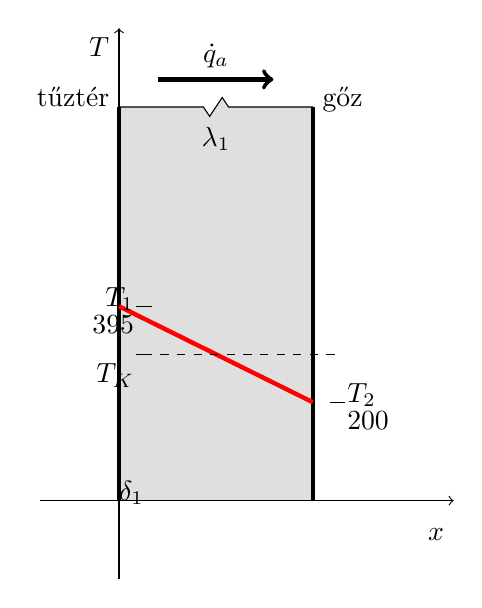
\begin{tikzpicture}
			\pgfmathsetmacro{\d}{16/6.5}
			\pgfmathsetmacro{\L}{5}
			\pgfmathsetmacro{\TA}{395/160}
			\pgfmathsetmacro{\TB}{200/160}
			\pgfmathsetmacro{\TK}{(\TA+\TB)/2}
			
			% Fal
			\fill[gray,opacity=0.25] (0,0) -- (0,\L) -- ({\d/2-0.16},\L) -- ({\d/2-0.08}, {\L-0.12}) -- ({\d/2+0.08}, {\L +0.12}) -- ({\d/2+0.16}, \L) -- (\d, \L) -- (\d, 0);
			\draw[] (0,\L) -- ({\d/2-0.16},\L) -- ({\d/2-0.08}, {\L-0.12}) -- ({\d/2+0.08}, {\L+0.12}) -- ({\d/2+0.16}, \L) -- (\d, \L);
			\draw[ultra thick] (0,0) -- (0,\L);
			\draw[ultra thick] (\d, 0) -- (\d, \L);
			
			% Feliratok
			\node[anchor=base east] at (0, \L) {tűztér};
			\node[anchor=base west] at (\d, \L) {gőz};
			
			% Tengelyek
			\draw[->] (0,-1) -- (0,\L+1) node[anchor=north east]{$T$};
			\draw[->] (-1,0) -- (4.25,0) node[anchor=base east, shift={(0,-0.5)}]{$x$};
			
			% Hőáram és hőáramsűrűség
			\draw[->, ultra thick] (0.5,{\L+0.35}) -- ({\d/2},{\L+0.35}) node[anchor=south]{$\dot{q}_a$} -- ({\d - 0.5},{\L+0.35});
			
			% A hővezetési tényező
			\node[anchor=base] at ({\d/2},{\L-0.5}) {$\lambda_1$};
			
			% T(x)
			\draw[red, ultra thick] (0,\TA) -- (\d,\TB);
			
			% A delta_1 falvastagság
			\pgflength[xa=0, ya=0, xb=\d, yb=0, alim=0]{$\delta_1$};
			
			% A hőmérséklet értékek
			\draw (-0.1,\TA) -- (0.1,\TA);
			\node[anchor=base east] at (0,\TA) {$T_1$};
			\node[anchor=north east] at (0,\TA) {$\SI{395}{\celsius}$};
			
			\draw (-0.1+\d,\TB) -- (0.1+\d,\TB);
			\node[anchor=base west] at (\d,\TB) {$T_2$};
			\node[anchor=north west] at (\d,\TB) {$\SI{200}{\celsius}$};
			
			% A közepes hőmérséklet
			\draw[dashed] (0,\TK) -- (\d,\TK);
			\draw (-0.1,\TK) -- (0.1,\TK);
			\node[anchor=north east] at (0,\TK) {$T_K$};
			
		\end{tikzpicture}
		\caption{A hőmérséklet-hely függvény az a) esetben.}
	\end{subfigure}
	\begin{subfigure}[b]{0.31\textwidth}
		\centering
		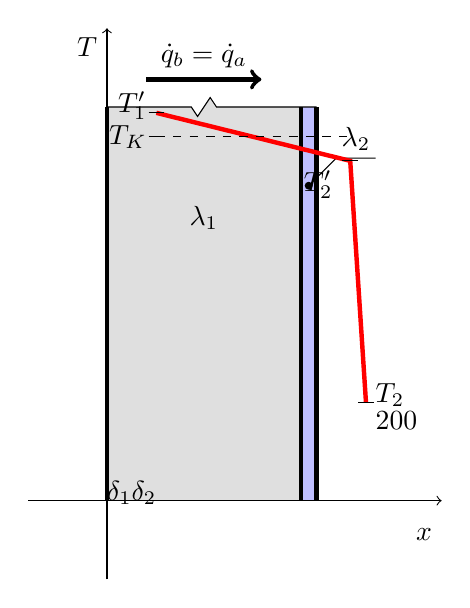
\begin{tikzpicture}
			\pgfmathsetmacro{\d}{16/6.5}
			\pgfmathsetmacro{\v}{1.2/6}
			\pgfmathsetmacro{\L}{5}
			\pgfmathsetmacro{\TA}{788/160}
			\pgfmathsetmacro{\TB}{690.5/160}
			\pgfmathsetmacro{\TC}{200/160}
			\pgfmathsetmacro{\TK}{(\TA+\TB)/2}
			
			% Fal
			\fill[gray,opacity=0.25] (0,0) -- (0,\L) -- ({\d/2-0.16},\L) -- ({\d/2-0.08}, {\L-0.12}) -- ({\d/2+0.08}, {\L +0.12}) -- ({\d/2+0.16}, \L) -- (\d, \L) -- (\d, 0);
			\fill[blue,opacity=0.25] (\d, \L) -- (\d, 0) -- (\d+\v, 0) -- (\d+\v, \L);
			\draw[] (0,\L) -- ({\d/2-0.16},\L) -- ({\d/2-0.08}, {\L-0.12}) -- ({\d/2+0.08}, {\L+0.12}) -- ({\d/2+0.16}, \L) -- (\d, \L) -- (\d+\v, \L);
			\draw[ultra thick] (0,0) -- (0,\L);
			\draw[ultra thick] (\d, 0) -- (\d, \L);
			\draw[ultra thick] (\d+\v, 0) -- (\d+\v, \L);
			
			% Tengelyek
			\draw[->] (0,-1) -- (0,\L+1) node[anchor=north east]{$T$};
			\draw[->] (-1,0) -- (4.25,0) node[anchor=base east, shift={(0,-0.5)}]{$x$};
			
			% Hőáram és hőáramsűrűség
			\draw[->, ultra thick] (0.5,{\L+0.35}) -- ({\d/2},{\L+0.35}) node[anchor=south]{$\dot{q}_b = \dot{q}_a$} -- ({\d - 0.5},{\L+0.35});
			
			% A hővezetési tényező
			\node[anchor=base] at ({\d/2},{\L-1.5}) {$\lambda_1$};
			\node[anchor=base] at ({\d+\v+0.5},{\L-0.5}) {$\lambda_2$};
			\draw ({\d+\v+0.75},{\L-0.65}) -- ({\d+\v+0.25},{\L-0.65}) -- ({\d+\v/2},{\L-1});
			\fill[] ({\d+\v/2},{\L-1}) circle[radius=0.05];
			
			% A falvastagságok
			\pgflength[xa=0, ya=0, xb=\d, yb=0, alim=0]{$\delta_1$};
			\pgflength[xa=\d, ya=0, xb=\d+\v, yb=0, alim=0, a=0, belül=2]{$\delta_2$};
			
			% T(x)
			\draw[red, ultra thick] (0,\TA) -- (\d,\TB) -- (\d+\v,\TC);
			
			% Falhőmérsékletek
			\draw (-0.1,\TA) -- (0.1,\TA);
			\node[anchor=base east] at (0,\TA) {$T_1'$};
			
			\draw (-0.1+\d,\TB) -- (0.1+\d,\TB);
			\node[anchor=north east] at (\d-0.1,\TB) {$T_2'$};
			
			\draw (-0.1+\d+\v,\TC) -- (0.1+\d+\v,\TC);
			\node[anchor=base west] at (\d+\v,\TC) {$T_2$};
			\node[anchor=north west] at (\d+\v,\TC) {$\SI{200}{\celsius}$};
			
			% A közepes hőmérséklet
			\draw[dashed] (0,\TK) -- (\d,\TK);
			\draw (-0.1,\TK) -- (0.1,\TK);
			\node[anchor=east] at (0,\TK) {$T_K$};
			
		\end{tikzpicture}
		\caption{A hőmérséklet-hely függvény az b) esetben.}
	\end{subfigure}
	\begin{subfigure}[b]{0.31\textwidth}
		\centering
		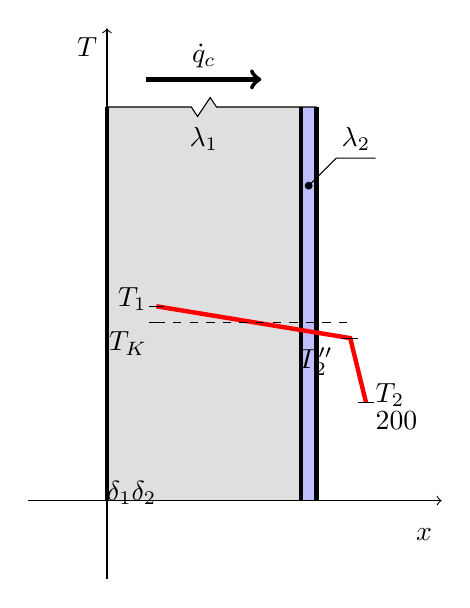
\begin{tikzpicture}
			\pgfmathsetmacro{\d}{16/6.5}
			\pgfmathsetmacro{\v}{1.2/6}
			\pgfmathsetmacro{\L}{5}
			\pgfmathsetmacro{\TA}{395/160}
			\pgfmathsetmacro{\TB}{330.3/160}
			\pgfmathsetmacro{\TC}{200/160}
			\pgfmathsetmacro{\TK}{(\TA+\TB)/2}
			
			% Fal
			\fill[gray,opacity=0.25] (0,0) -- (0,\L) -- ({\d/2-0.16},\L) -- ({\d/2-0.08}, {\L-0.12}) -- ({\d/2+0.08}, {\L +0.12}) -- ({\d/2+0.16}, \L) -- (\d, \L) -- (\d, 0);
			\fill[blue,opacity=0.25] (\d, \L) -- (\d, 0) -- (\d+\v, 0) -- (\d+\v, \L);
			\draw[] (0,\L) -- ({\d/2-0.16},\L) -- ({\d/2-0.08}, {\L-0.12}) -- ({\d/2+0.08}, {\L+0.12}) -- ({\d/2+0.16}, \L) -- (\d, \L) -- (\d+\v, \L);
			\draw[ultra thick] (0,0) -- (0,\L);
			\draw[ultra thick] (\d, 0) -- (\d, \L);
			\draw[ultra thick] (\d+\v, 0) -- (\d+\v, \L);
			
			% Tengelyek
			\draw[->] (0,-1) -- (0,\L+1) node[anchor=north east]{$T$};
			\draw[->] (-1,0) -- (4.25,0) node[anchor=base east, shift={(0,-0.5)}]{$x$};
			
			% Hőáram és hőáramsűrűség
			\draw[->, ultra thick] (0.5,{\L+0.35}) -- ({\d/2},{\L+0.35}) node[anchor=south]{$\dot{q}_c$} -- ({\d - 0.5},{\L+0.35});
			
			% A hővezetési tényező
			\node[anchor=base] at ({\d/2},{\L-0.5}) {$\lambda_1$};
			\node[anchor=base] at ({\d+\v+0.5},{\L-0.5}) {$\lambda_2$};
			\draw ({\d+\v+0.75},{\L-0.65}) -- ({\d+\v+0.25},{\L-0.65}) -- ({\d+\v/2},{\L-1});
			\fill[] ({\d+\v/2},{\L-1}) circle[radius=0.05];
			
			% A falvastagságok
			\pgflength[xa=0, ya=0, xb=\d, yb=0, alim=0]{$\delta_1$};
			\pgflength[xa=\d, ya=0, xb=\d+\v, yb=0, alim=0, a=0, belül=2]{$\delta_2$};
			
			% T(x)
			\draw[red, ultra thick] (0,\TA) -- (\d,\TB) -- (\d+\v,\TC);
			
			% Falhőmérsékletek
			\draw (-0.1,\TA) -- (0.1,\TA);
			\node[anchor=base east] at (0,\TA) {$T_1$};
			%\node[anchor=north east] at (0,\TA) {$\SI{395}{\celsius}$};
			
			\draw (-0.1+\d,\TB) -- (0.1+\d,\TB);
			\node[anchor=north east] at (\d-0.1,\TB) {$T_2''$};
			
			\draw (-0.1+\d+\v,\TC) -- (0.1+\d+\v,\TC);
			\node[anchor=base west] at (\d+\v,\TC) {$T_2$};
			\node[anchor=north west] at (\d+\v,\TC) {$\SI{200}{\celsius}$};
			
			% A közepes hőmérséklet
			\draw[dashed] (0,\TK) -- (\d,\TK);
			\draw (-0.1,\TK) -- (0.1,\TK);
			\node[anchor=north east] at (0,\TK) {$T_K$};
			
		\end{tikzpicture}
		\caption{A hőmérséklet-hely függvény a c) esetben.}
	\end{subfigure}
\end{figure}

\subsubsection*{a) Határozzuk meg a fal közepes hőmérsékletét és a falban kialakuló hőáramsűrűséget!}

A fal közepes hőmérséklete a lineáris hőmérsékleteloszlás miatt a falhőmérsékletek átlaga:
\begin{equation}
	T_K = \frac{T_1 + T_2}{2} = \SI{297.5}{\celsius}
\end{equation}

Nem lineáris hőmérsékleteloszlás esetén a hőmérséklet-hely függvény határozott integráljának és a falvastagságnak a hányadosa a közepes hőmérséklet.

A hőáramsűrűség a falban
\begin{equation}
	\dot{q}_a = \frac{\lambda_1}{\delta_1} (T_1 - T_2) = \SI{524}{\kilo\watt\per\meter\squared}
\end{equation}
Ebben a feladatban a kazánfal oldalain végbemenő hőátadást tökéletesnek tekintjük, azaz a falhőmérsékletek megegyeznek a közeghőmérsékletekkel.

\subsubsection*{b) A kazán falára $\delta_2 = \SI{1.2}{\milli\meter}$ vastag kazánkőréteg rakódik. Változatlan gőztermelés és gőznyomás esetén számítsuk ki a kazán falának közepes hőmérsékletét!}

A vízkőréteg hővezetési tényezője $\lambda_2 = \SI{1.6}{\watt\per\meter\kelvin}$.

\vspace{2mm}

A "változatlan gőztermelés" kifejezés azt jelenti, hogy a gőzoldali falhőmérséklet és a hőáramsűrűség a falban nem változik. A vízkőréteg miatt a hőáramsűrűség csak úgy maradhat azonos $\dot{q}_a$-val, hogy a tűztér oldali $T_1'$ falhőmérséklet sokkal nagyobb $T_1$-nél, a $T_2'$ falhőmérséklet pedig nem azonos a gőzoldali $T_2$ hőmérséklettel. A vízkőréteg hővezetési tényezője sokkal kisebb a kazánlemezénél, ezért a kisebb rétegvastagság ellenére nagyobb hőmérséklet esik rajta.

A fal közepes hőmérséklete itt is a két falhőmérséklet átlaga:
\begin{equation}
	T_K' = \frac{T_1' + T_2'}{2}
\end{equation}

A $T_1'$ és a $T_2'$ falhőmérséklet a $q_b$ hőáramsűrűség alapján számítható ki:
\begin{equation}
	\dot{q}_b = \dot{q}_a = \frac{\lambda_1}{\delta_1} (T_1' - T_2') = \frac{\lambda_2}{\delta_2} (T_2' - T_2)
\end{equation}

\begin{equation}
	T_2' = T_2 + \frac{\delta_2}{\lambda_2}\dot{q}_a = \SI{200}{\celsius} + \frac{\SI{1.2}{\milli\meter}}{\SI{1.6}{\watt\per\meter\kelvin}} \SI{524}{\kilo\watt\per\meter\squared} = \SI{593}{\celsius}
\end{equation}

\begin{equation}
	T_1' = T_2' + \frac{\delta_1}{\lambda_1}\dot{q}_a = \SI{593}{\celsius} + \frac{\SI{16}{\milli\meter}}{\SI{43}{\watt\per\meter\kelvin}} \SI{524}{\kilo\watt\per\meter\squared} = \SI{788}{\celsius}
\end{equation}

\subsubsection*{c) Ha szilárdsági okok miatt a fal hőmérséklete nem emelkedhet, de a gőznyomás változatlan, mekkora lesz a hőáramsűrűség?}

Ha gőznyomás nem változik, akkor a gőz hőmérséklete sem változik, mivel a kazánban a nedves gőzmezőbe eső állapotú a víz, és ott T--s diagram szerint az izotermák és az izobár vonalak egybeesnek. Tehát a gőzoldali hőmérséklet $T_2$. Ha szilárdsági okok miatt a fal hőmérséklete nem emelkedhet, akkor a tűztér oldali hőmérséklet az eredeti $T_1$.

A $\dot{q}_c$ hőáramsűrűség azonos a kazánfalban és a vízkőrétegben:
\begin{equation}
	\dot{q}_c = \frac{\lambda_1}{\delta_1} (T_1 - T_2'') = \frac{\lambda_2}{\delta_2} (T_2'' - T_2)
\end{equation}

Kifejezve a két hőmérsékletkülönbséget, és összeadva a két egyenletet:
\begin{equation}
	\left.
	\begin{array}{lcl}
		\dot{q}_c \dfrac{\delta_1}{\lambda_1} = (T_1 - T_2'') \\
		\dot{q}_c \dfrac{\delta_2}{\lambda_2} = (T_2'' - T_2)
	\end{array}
	\right\rbrace
	\quad \Rightarrow \quad 
	\dot{q}_c \left(\dfrac{\delta_1}{\lambda_1} + \dfrac{\delta_2}{\lambda_2} \right) = (T_1 - T_2) 
	\quad \Rightarrow \quad 
	\dot{q}_c = 
	\SI{173.78}{\kilo\watt\per\meter\squared}
\end{equation}

A fenti két egyenletet kétismeretlenes egyenletrendszernek is tekinthetjük, ahol a hőáramsűrűség mellett a másik ismeretlen a $T_2''$ falhőmérséklet. A hőáramsűrűséget visszahelyettesítve megkaphatjuk az értékét:
\begin{equation}
	T_2'' = T_1 - \dot{q}_c \dfrac{\delta_1}{\lambda_1} = \SI{330.34}{\celsius}
\end{equation}

\pagebreak



% K5/2-es feladat


\section*{K5/2. feladat: Szénacél csőre kifagyó jégréteg}
\addcontentsline{toc}{section}{K5/2. feladat: Szénacél csőre kifagyó jégréteg}

\begin{tabular}{ | p{2cm} | p{14cm} | } 
	\hline
	Név & Szalay István \\ 
	\hline
	Szak & \\ 
	\hline
	Félév & 2019/2020 II. (tavaszi) félév \\ 
	\hline
\end{tabular}
\vspace{0.5cm}

\noindent Egy NÁ125-ös szénacél csőben (a külső átmérő $d_2 = \SI{133}{\milli\meter}$, a belső átmérő $d_1 = \SI{125}{\milli\meter}$, a falvastagság $s = \SI{4}{\milli\meter}$) ammóniát szállítanak, amelynek nyomása $p = \SI{2.9}{\bar}$, hőmérséklete $T_1 = \SI{-10}{\celsius}$.

A környezet levegője ($T_4 = \SI{+10}{\celsius}$) melegíti a csövet, ammónia forrásban van a cső belsejében, így belülről hőelvonás van, és a cső hideg külső felületére kifagy a levegő nedvességtartalma. A kifagyott jégréteg szigetelőként működik, beáll az egyensúlyi állapot.

Meghatározandó a csőre fagyott jégréteg külső $d_3$ átmérője! A jégréteg felületének hőmérséklete $T_3 = \SI{0}{\celsius}$ (olvadó jég), a csőfal belső hőmérséklete pedig a forrásban lévő ammónia jó hőátadási tényezője miatt $T_1 = \SI{-10}{\celsius}$-nak vehető (a hőátadás termikus ellenállása elhanyagolható).

\begin{figure}[h]
	\centering
	\begin{tikzpicture}
		% Fiktív értékek a vázlathoz
		\pgfmathsetmacro{\DB}{4}
		\pgfmathsetmacro{\DK}{6}
		\pgfmathsetmacro{\DJ}{9}
		\pgfmathsetmacro{\lambdaA}{8}
		\pgfmathsetmacro{\lambdaJ}{2.9}
		\pgfmathsetmacro{\alfaL}{11.5}
		\pgfmathsetmacro{\qlin}{326.815}
		
		\pgfmathsetmacro{\RA}{\DB/2}
		\pgfmathsetmacro{\RB}{\DK/2}
		\pgfmathsetmacro{\RC}{\DJ/2}
		
		\pgfmathsetmacro{\L}{3}
		
		\pgfmathsetmacro{\kelvin}{4.2}
		\pgfmathsetmacro{\TA}{-10/\kelvin}
		\pgfmathsetmacro{\TB}{-7.36/\kelvin}
		\pgfmathsetmacro{\TC}{0/\kelvin}
		\pgfmathsetmacro{\TD}{10/\kelvin}
		
		% KÖRBEVÁGÁS
		\clip ({-1.25}, {-(\L)-2}) rectangle ({2.2*\RC}, {\L+1});
		
		% A csőfal és a jégréteg
		\fill[gray, opacity=0.25] (\RA,\L) -- ({(\RA+\RB)/2-0.16},\L) -- ({(\RA+\RB)/2-0.08}, {\L-0.12}) -- ({(\RA+\RB)/2+0.08}, {\L+0.12}) -- ({(\RA+\RB)/2+0.16}, \L) -- (\RB, \L) -- (\RB, -\L) -- ({(\RA+\RB)/2+0.16}, -\L) -- ({(\RA+\RB)/2+0.08}, {-\L+0.12}) -- ({(\RA+\RB)/2-0.08}, {-\L-0.12}) -- ({(\RA+\RB)/2-0.16},-\L) -- (\RA,-\L);
		\draw[] (\RA,\L) -- ({(\RA+\RB)/2-0.16},\L) -- ({(\RA+\RB)/2-0.08}, {\L-0.12}) -- ({(\RA+\RB)/2+0.08}, {\L+0.12}) -- ({(\RA+\RB)/2+0.16}, \L) -- (\RB, \L);
		\draw[] (\RA,-\L) -- ({(\RA+\RB)/2-0.16},-\L) -- ({(\RA+\RB)/2-0.08}, {-\L-0.12}) -- ({(\RA+\RB)/2+0.08}, {-\L+0.12}) -- ({(\RA+\RB)/2+0.16}, -\L) -- (\RB, -\L);
		
		\fill[blue, opacity=0.25] (\RB,\L) -- ({(\RB+\RC)/2-0.16},\L) -- ({(\RB+\RC)/2-0.08}, {\L-0.12}) -- ({(\RB+\RC)/2+0.08}, {\L+0.12}) -- ({(\RB+\RC)/2+0.16}, \L) -- (\RC, \L) -- (\RC, -\L) -- ({(\RB+\RC)/2+0.16}, -\L) -- ({(\RB+\RC)/2+0.08}, {-\L+0.12}) -- ({(\RB+\RC)/2-0.08}, {-\L-0.12}) -- ({(\RB+\RC)/2-0.16},-\L) -- (\RB,-\L);
		\draw[] (\RB,\L) -- ({(\RB+\RC)/2-0.16},\L) -- ({(\RB+\RC)/2-0.08}, {\L-0.12}) -- ({(\RB+\RC)/2+0.08}, {\L+0.12}) -- ({(\RB+\RC)/2+0.16}, \L) -- (\RC, \L);
		\draw[] (\RB,-\L) -- ({(\RB+\RC)/2-0.16},-\L) -- ({(\RB+\RC)/2-0.08}, {-\L-0.12}) -- ({(\RB+\RC)/2+0.08}, {-\L+0.12}) -- ({(\RB+\RC)/2+0.16}, -\L) -- (\RC, -\L);
		
		\draw[ultra thick] (\RA,-\L) -- (\RA,\L);
		\draw[ultra thick] (\RB,-\L) -- (\RB,\L);
		\draw[ultra thick] (\RC,-\L) -- (\RC,\L);
		
		% Tengelyek
		\draw[->] (0,-\L) -- (0,\L+1) node[anchor=north east]{$T$};
		\draw[->] (-1.25, 0) -- (\RC+3, 0) node[anchor=base east, shift={(0,-0.5)}]{$r$};
		
		% Hőáram és hőáramsűrűség
		\draw[->, ultra thick] (\RC-0.2,{\L+0.35}) -- ({(\RA+\RC)/2},{\L+0.35}) node[anchor=south]{$\dot{q}_{lin}$} -- (\RA+0.2,{\L+0.35});
		\draw[->, ultra thick] (\RC+2.2,{\L+0.35}) -- (\RC+1.2,{\L+0.35}) node[anchor=south]{$\dot{q}_{\acute{a}t}$} -- (\RC+0.2,{\L+0.35});
		
		% A hővezetési és hőátadási tényezők
		\node[anchor=base] at ({(\RA+\RB)/2},{\L-0.5}) {$\lambda_1$};
		\node[anchor=base] at ({(\RB+\RC)/2},{\L-0.5}) {$\lambda_2$};
		\node[anchor=base west] at ({(\RC+0.1},{\L-0.5}) {$\alpha$};
		
		% Az átmérők
		\pgflength[xa={-\RA}, ya={-\L}, xb={\RA}, yb={-\L}, alim=0, blim=1, ra=0.6]{$\diameter d_1$};
		\pgflength[xa={-\RB}, ya={-\L}, xb={\RB}, yb={-\L}, alim=0, blim=1, ra=1.2]{$\diameter d_2$};
		\pgflength[xa={-\RC}, ya={-\L}, xb={\RC}, yb={-\L}, alim=0, blim=1, ra=1.8]{$\diameter d_3$};
		
		% T(r) körülbelüli hőmérséklet-hely függvény
		\draw[red, ultra thick] (0.5,\TA) -- (\RA,\TA);
		\draw[ultra thick, color=red, domain=\RA:\RB, smooth, variable=\r] plot (\r, {\TA + ( \qlin/(2*3.14159*\lambdaA) * ln(2*\r/\DB))/\kelvin});
		\draw[ultra thick, color=red, domain=\RB:\RC, smooth, variable=\r] plot (\r, {\TA + (\qlin/(2*3.14159*\lambdaA) * ln(\DK/\DB) + \qlin/(2*3.14159*\lambdaJ) * ln(2*\r/\DK))/\kelvin});
		
		\draw[ultra thick, color=red, domain=\RC:1.5*\RC, smooth, variable=\r] plot (\r, {\TD * (1-exp(-(\r-\RC)/0.5))});
		
		% A hőmérséklet értékek
		\draw (-0.1,\TA) -- (0.1,\TA);
		\node[anchor=base east] at (0,\TA) {$T_1$};
		\node[anchor=north east] at (0,\TA) {$\SI{-10}{\celsius}$};
		
		\draw (-0.1,\TB) -- (0.1,\TB);
		\draw[black, opacity=0.5, dashed] (0,\TB) -- (\RB,\TB);
		\node[anchor=base east] at (0,\TB) {$T_2$};
		
		\draw (-0.1,\TD) -- (0.1,\TD);
		\draw[black, opacity=0.5, dashed] (0,\TD) -- (1.5*\RC,\TD);
		\node[anchor=base east] at (0,\TD) {$T_4$};
		\node[anchor=north east] at (0,\TD) {$\SI{10}{\celsius}$};
		
		\node[anchor=north west] at (\RC,\TC) {$T_3$};
		\node[anchor=north west] at (\RC, -0.45) {$\SI{0}{\celsius}$};
		
		% Feliratok
		\node[anchor=base east] at (\RA, \L) {ammónia};
		\node[anchor=base west] at (\RC, -\L) {levegő};
		
		% Adatok
		\node[anchor=base west] at (1.6*\RC, \L) {$\lambda_1 = \SI{45}{\watt\per\meter\kelvin}$};
		\node[anchor=base west] at (1.6*\RC, 0.65*\L) {$\lambda_2 = \SI{2.32}{\watt\per\meter\kelvin}$};
		\node[anchor=base west] at (1.6*\RC, 0.3*\L) {$\alpha = \SI{11.5}{\watt\per\meter\squared\kelvin}$};
		
	\end{tikzpicture}
	\caption{A hőmérséklet-hely függvény \textbf{nem méretarányos} vázlata.}
\end{figure}

\subsubsection*{Vizsgálat többrétegű hengeres falként}
A csőfal és a rárakódó jégréteg hengeres alakú, ezért lineáris a hőáramsűrűségeket tudjuk felírni. A csőfalban és a jégrétegben állandósult a hőmérsékleteloszlás és csak hővezetés történik. A hengeres falakra a $\dot{q}_{lin}$ \textbf{vezetéses} lineáris hőáramsűrűség vonatkozik.
\begin{equation}
	\dot{q}_{lin} = \dfrac{T_3 - T_1}{\dfrac{\ln\frac{d_2}{d_1}}{2 \pi \lambda_1} + \dfrac{\ln\frac{d_3}{d_2}}{2 \pi \lambda_2}}
\end{equation}

A levegőből a jégrétegbe \textbf{átadódó} $\dot{q}_{\acute{a}t}$ lineáris hőáramsűrűség: 
\begin{equation}
	\dot{q}_{\acute{a}t} = \alpha d_3 \pi (T_4 - T_3)
\end{equation}

A két lineáris hőáramsűrűséget az ábrán úgy vettük fel, hogy a hőmérsékletcsökkenés irányába pozitívak, ezért a felírásuknál a nagyobb hőmérsékletből vonjuk ki a kisebbet.

Az energiamegmaradás miatt a két lineáris hőáramsűrűség egyenlő:
\begin{equation}
	\dot{q}_{lin} = \dot{q}_{\acute{a}t} = \dot{q}
\end{equation}

A fentiekből az alábbi kétismeretlenes egyenletrendszert kapjuk, amiben a jégréteg $d_3$ átmérője a a $\dot{q}$ lineáris hőáramsűrűség az ismeretlenek. Az egyenletrendszer nem lineáris, átrendezéssel nem oldható meg (transzcendens), csak numerikus közelítő megoldása lehetséges:
\begin{equation}
	\left.
	\begin{array}{lcl}
		\dot{q} = \dfrac{T_3 - T_1}{\dfrac{\ln\frac{d_2}{d_1}}{2 \pi \lambda_1} + \dfrac{\ln\frac{d_3}{d_2}}{2 \pi \lambda_2}} \\ \\
		\dot{q} = \alpha d_3 \pi (T_4 - T_3)
	\end{array}
	\right\rbrace
	\quad \Rightarrow \quad 
	\left\lbrace
	\begin{array}{lcl}
		\dot{q} \approx \SI{137.873}{\watt\per\meter} \\ \\
		d_3 \approx \SI{381.6}{\milli\meter}
	\end{array}
	\right.
\end{equation}

Innen a jégréteg vastagsága $\dfrac{1}{2}\left(d_3 - d_2\right) = \SI{124.3}{\milli\meter}$.

\subsubsection*{A méretarányos ábra és a hőmérséklet hely függvény}
A lineáris hőáramsűrűség és a jég külső átmérőjének numerikus közelítő megoldását felhasználva megrajzolható méretarányosan a $T\!\left(r\right)$ hőmérséklet-hely függvény. A hőmérséklet a $d_1$ átmérőn belül állandó $T_1$ érték. A csőfalban és a jégrétegben $T\!\left(r\right) = T_0 + \dfrac{\dot{q}}{2 \pi \lambda} \ln\dfrac{r}{r_0}$ alakban írható fel, ahol a $T_0$ a belső $r_0$ sugárhoz tartozó hőmérséklet.

A csőfal esetén $T_0 = T_1$ és $r_0 = \dfrac{d_1}{2}$:
\begin{equation}
	T\!\left(r\right) = T_1 + \dfrac{\dot{q}}{2 \pi \lambda_1} \ln\dfrac{2 r}{d_1}
\end{equation}

Innen megkaphatjuk a csőfal és a jégréteg határfelületének hőmértékletét, $T_2$-t:
\begin{equation}
	T_2 = T\!\left(\frac{d_2}{2}\right) = T_1 + \dfrac{\dot{q}}{2 \pi \lambda_1} \ln\dfrac{d_2}{d_1} = \SI{-9.96}{\celsius}
\end{equation}

A jégréteg esetén $T_0 = T_2$ és $r_0 = \dfrac{d_2}{2}$:
\begin{equation}
	T\!\left(r\right) = T_2 + \dfrac{\dot{q}}{2 \pi \lambda_2} \ln\dfrac{2 r}{d_2}
\end{equation}


\begin{figure}[h]
	\centering
	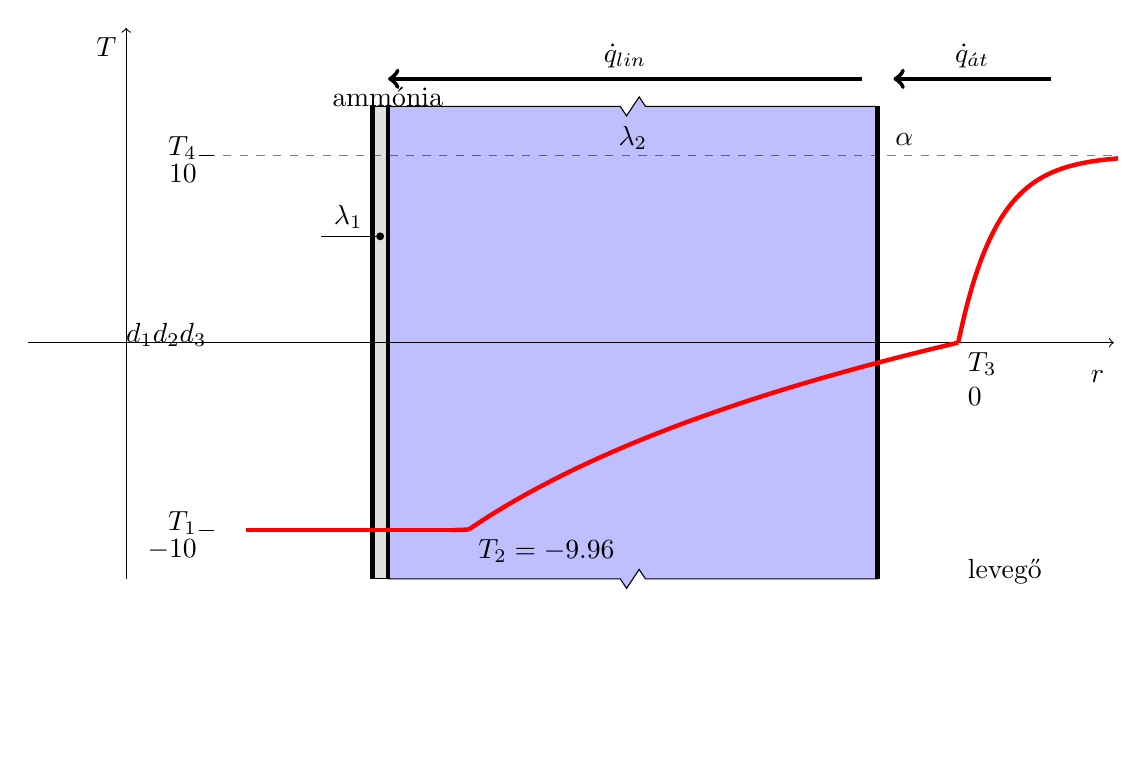
\begin{tikzpicture}
		% Fiktív értékek a vázlathoz
		\pgfmathsetmacro{\meter}{1/50}
		\pgfmathsetmacro{\DB}{0.125/\meter}
		\pgfmathsetmacro{\DK}{0.133/\meter}
		\pgfmathsetmacro{\DJ}{0.3816/\meter}
		\pgfmathsetmacro{\lambdaA}{45}
		\pgfmathsetmacro{\lambdaJ}{2.32}
		\pgfmathsetmacro{\alfaL}{11.5}
		\pgfmathsetmacro{\qlin}{137.873}
		
		\pgfmathsetmacro{\RA}{\DB/2}
		\pgfmathsetmacro{\RB}{\DK/2}
		\pgfmathsetmacro{\RC}{\DJ/2}
		
		\pgfmathsetmacro{\L}{3}
		
		\pgfmathsetmacro{\kelvin}{4.2}
		\pgfmathsetmacro{\TA}{-10/\kelvin}
		\pgfmathsetmacro{\TB}{-9.96/\kelvin}
		\pgfmathsetmacro{\TC}{0/\kelvin}
		\pgfmathsetmacro{\TD}{10/\kelvin}
		
		% KÖRBEVÁGÁS
		\clip ({-1.25}, {-(\L)-2}) rectangle ({1.32*\RC}, {\L+1});
		
		% A csőfal és a jégréteg
		\fill[gray,opacity=0.25] (\RA,\L) -- (\RB, \L) -- (\RB, -\L) -- (\RA,-\L);
		\draw[] (\RA,\L) -- (\RB, \L);
		\draw[] (\RA,-\L) -- (\RB, -\L);
		
		\fill[blue,opacity=0.25] (\RB,\L) -- ({(\RB+\RC)/2-0.16},\L) -- ({(\RB+\RC)/2-0.08}, {\L-0.12}) -- ({(\RB+\RC)/2+0.08}, {\L+0.12}) -- ({(\RB+\RC)/2+0.16}, \L) -- (\RC, \L) -- (\RC, -\L) -- ({(\RB+\RC)/2+0.16}, -\L) -- ({(\RB+\RC)/2+0.08}, {-\L+0.12}) -- ({(\RB+\RC)/2-0.08}, {-\L-0.12}) -- ({(\RB+\RC)/2-0.16},-\L) -- (\RB,-\L);
		\draw[] (\RB,\L) -- ({(\RB+\RC)/2-0.16},\L) -- ({(\RB+\RC)/2-0.08}, {\L-0.12}) -- ({(\RB+\RC)/2+0.08}, {\L+0.12}) -- ({(\RB+\RC)/2+0.16}, \L) -- (\RC, \L);
		\draw[] (\RB,-\L) -- ({(\RB+\RC)/2-0.16},-\L) -- ({(\RB+\RC)/2-0.08}, {-\L-0.12}) -- ({(\RB+\RC)/2+0.08}, {-\L+0.12}) -- ({(\RB+\RC)/2+0.16}, -\L) -- (\RC, -\L);
		
		\draw[ultra thick] (\RA,-\L) -- (\RA,\L);
		\draw[ultra thick] (\RB,-\L) -- (\RB,\L);
		\draw[ultra thick] (\RC,-\L) -- (\RC,\L);
		
		% Tengelyek
		\draw[->] (0,-\L) -- (0,\L+1) node[anchor=north east]{$T$};
		\draw[->] (-1.25, 0) -- (\RC+3, 0) node[anchor=base east, shift={(0,-0.5)}]{$r$};
		
		% Hőáram és hőáramsűrűség
		\draw[->, ultra thick] (\RC-0.2,{\L+0.35}) -- ({(\RA+\RC)/2},{\L+0.35}) node[anchor=south]{$\dot{q}_{lin}$} -- (\RA+0.2,{\L+0.35});
		\draw[->, ultra thick] (\RC+2.2,{\L+0.35}) -- (\RC+1.2,{\L+0.35}) node[anchor=south]{$\dot{q}_{\acute{a}t}$} -- (\RC+0.2,{\L+0.35});
		
		% A hővezetési és hőátadási tényezők
		\node[anchor=base east] at ({\RA},{\L-1.5}) {$\lambda_1$};
		\draw ({\RA-0.65},{\L-1.65}) -- ({(\RA+\RB)/2},{\L-1.65});
		\fill[] ({(\RA+\RB)/2},{\L-1.65}) circle[radius=0.05];
		
		\node[anchor=base] at ({(\RB+\RC)/2},{\L-0.5}) {$\lambda_2$};
		\node[anchor=base west] at ({(\RC+0.1},{\L-0.5}) {$\alpha$};
		
		% Az átmérők
		\pgflength[xa={-\RA}, ya={-\L}, xb={\RA}, yb={-\L}, alim=0, blim=1, ra=0.6]{$\diameter d_1$};
		\pgflength[xa={-\RB}, ya={-\L}, xb={\RB}, yb={-\L}, alim=0, blim=1, ra=1.2]{$\diameter d_2$};
		\pgflength[xa={-\RC}, ya={-\L}, xb={\RC}, yb={-\L}, alim=0, blim=1, ra=1.8]{$\diameter d_3$};
		
		% A T(r) VALÓS hőmérséklet-hely függvény
		\draw[red, ultra thick] (0.5,\TA) -- (\RA,\TA);
		
		\draw[ultra thick, color=red, domain=\RA:\RB, smooth, variable=\r] plot (\r, {\TA + ( \qlin/(2*3.14159*\lambdaA) * ln(2*\r/\DB))/\kelvin});
		
		\draw[ultra thick, color=red, domain=\RB:\RC, smooth, variable=\r] plot (\r, {\TA + (\qlin/(2*3.14159*\lambdaA) * ln(\DK/\DB) + \qlin/(2*3.14159*\lambdaJ) * ln(2*\r/\DK))/\kelvin});
		
		\draw[ultra thick, color=red, domain=\RC:1.25*\RC, smooth, variable=\r] plot (\r, {\TD * (1-exp(-(\r-\RC)/0.5))});
		
		% A hőmérséklet értékek
		\draw (-0.1,\TA) -- (0.1,\TA);
		\node[anchor=base east] at (0,\TA) {$T_1$};
		\node[anchor=north east] at (0,\TA) {$\SI{-10}{\celsius}$};
		
		\node[anchor=north west] at (\RB,\TB) {$T_2 = \SI{-9.96}{\celsius}$};
		
		\draw (-0.1,\TD) -- (0.1,\TD);
		\draw[black, opacity=0.5, dashed] (0,\TD) -- (1.25*\RC,\TD);
		\node[anchor=base east] at (0,\TD) {$T_4$};
		\node[anchor=north east] at (0,\TD) {$\SI{10}{\celsius}$};
		
		\node[anchor=north west] at (\RC,\TC) {$T_3$};
		\node[anchor=north west] at (\RC, -0.45) {$\SI{0}{\celsius}$};
		
		% Feliratok
		\node[anchor=base east] at (\RA, \L) {ammónia};
		\node[anchor=base west] at (\RC, -\L) {levegő};
		
	\end{tikzpicture}
	\caption{A hőmérséklet-hely függvény méretarányosan ábrázolva.}
\end{figure}


\subsubsection*{Vizsgálat többrétegű síkfalként}
A hengeres falon keresztül történő hőterjedés mindig közelíthető a hengeres fal kiterítésével kapott síkfalon át történő hőterjedéssel. A közelítés hibája a a hengeres fal vastagságától függ, minél vékonyabb, annál kisebb a síkfallal történő közelítés hibája.

A többrétegű hengeres falat többrétegű síkfallal közelíthetjük. A közelítő síkfal vastagsága és hossza megegyezik a hengeres réteg vastagságával és hosszával, a szélessége a hengeres réteg közepes átmérőjéhez tartozó kerülettel közelíthető:
\begin{equation}
	\left.
	\begin{array}{l}
		\dot{q}_{lin} = \dfrac{\lambda_1}{\frac{d_2-d_1}{2}} \dfrac{d_1+d_2}{2} \pi (T_2 - T_1) \\ \\
		\dot{q}_{lin} = \dfrac{\lambda_2}{\frac{d_3-d_2}{2}} \dfrac{d_2+d_3}{2} \pi (T_3 - T_2)
	\end{array}
	\right\rbrace
	\quad \Rightarrow \quad 
	\dot{q}_{lin} = \dfrac{T_3 - T_1}{
		\dfrac{d_2-d_1}{\lambda_1\left(d_1+d_2\right) \pi} + 
		\dfrac{d_3-d_2}{\lambda_2\left(d_2+d_3\right) \pi}
		}
\end{equation}

A falbeli lineáris hőáram és a hőátadást jellemző lineáris hőáram most is egyenlő. 
\begin{equation}
	\dot{q}_{lin} = \dfrac{T_3 - T_1}{
		\dfrac{d_2-d_1}{\lambda_1\left(d_1+d_2\right) \bcancel{\pi}} + 
		\dfrac{d_3-d_2}{\lambda_2\left(d_2+d_3\right)\bcancel{\pi}}
		}
	= 
	\alpha d_3 \bcancel{\pi} (T_4 - T_3) = \dot{q}_{\acute{a}t}
\end{equation}

Egyszerűsítve, és kifejezve a hőmérsékletkülönbségek hányadosát:
\begin{equation}
	\underbrace{\dfrac{T_3 - T_1}{T_4 - T_3}}_{\substack{T \\ \text{állandó}}}
	= 
	\underbrace{\dfrac{\left(d_2-d_1\right)\alpha}{\lambda_1\left(d_1+d_2\right)}}_{\substack{C \\ \text{állandó}}} d_3
	+ 
	\dfrac{\left(d_3-d_2\right) \alpha d_3}{\lambda_2\left(d_2+d_3\right)}
\end{equation}

Vezessük be a $T$ és $C$ állandókat, hogy gyorsabb és átláthatóbb legyen az egyenlet átrendezése:
\begin{equation}
	T = C d_3 +  \dfrac{\left(d_3-d_2\right) \alpha d_3}{\lambda_2\left(d_2+d_3\right)}
\end{equation}

Megszüntetve a törtet $d_3$-ra másodfokú egyenletet kapunk:
\begin{equation}
	T \lambda_2\left(d_2+d_3\right) = C d_3 \lambda_2\left(d_2+d_3\right) + \left(d_3-d_2\right) \alpha d_3
\end{equation}

\begin{equation}
	\SI{0}{\watt} = \left(C \lambda_2 +\alpha\right)d_3^2 + \left(C \lambda_2 d_2 - d_2 \alpha - T \lambda_2 \right) d_3 - T \lambda_2 d_2
\end{equation}

Innen a $d_3$ közelítő értéke:
\begin{equation}
	d_{3,1} = \SI{0.4008}{\meter}, 
	\quad 
	\underbrace{
		\left(d_{3,2} = \SI{-0.0668}{\meter}\right)
	}_{\substack{\text{a másodfokú egyenletnek megoldása,} \\ \text{de a fizikai problémának nem}}}
\end{equation}

A $d_3$ közelítő megoldással nyert értéke tehát \SI{400.8}{\milli\meter}. A nemlineáris egyenlet közelítő numerikus megoldásától ez 5\,\%-kal tér el.

\pagebreak


% K5/3-as feladat


% K5/4-es feladat


\section*{K5/4. feladat: Hengeres fal közelítése síkfallal}
\addcontentsline{toc}{section}{K5/4. feladat: Hengeres fal közelítése síkfallal}

\begin{tabular}{ | p{2cm} | p{14cm} | } 
	\hline
	Név & Szalay István \\ 
	\hline
	Szak & \\ 
	\hline
	Félév & 2019/2020 II. (tavaszi) félév \\ 
	\hline
\end{tabular}
\vspace{0.5cm}

\noindent Gyakorlati számítások során szokás a hengeres falon vezetéssel átjutó hőáramot közelítő módon síkfalra vonatkozó összefüggésekkel számolni. Határozza meg egy hengeres fal külső $d_2$ és belső $d_1$ átmérőjének hányadosa függvényében, hogy a lineáris hőáramsűrűség számításakor hány \%-os hibát vétünk az alábbi közelítő összefüggéseket használva:
\begin{equation}
	\dot{q}_{lin} = \dfrac{\lambda}{\delta} d_K \pi \left(T_1 - T_2\right),
	\quad 
	\delta = \dfrac{d_2 - d_1}{2}, 
	\quad 
	\text{és} 
	\quad d_K = \dfrac{d_1 + d_2}{2}
\end{equation}

ahol $\delta$ a falvastagság és $d_K$ a közepes átmérő.


\begin{figure}[h]
	\centering
	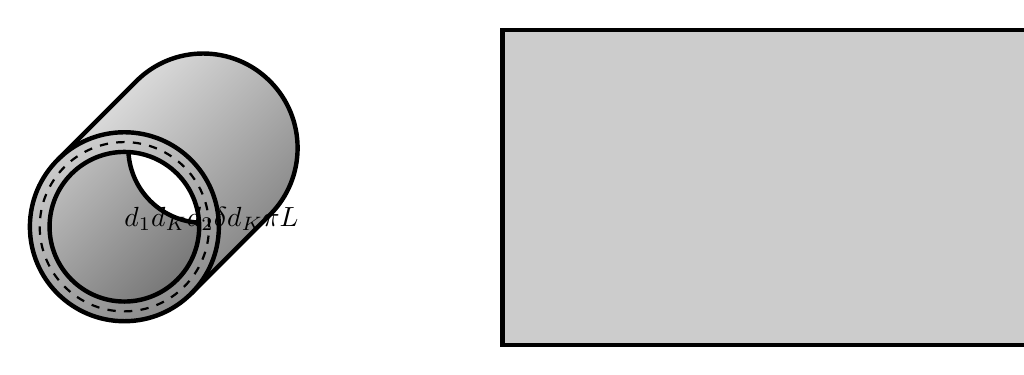
\begin{tikzpicture}
		\pgfmathsetmacro{\DB}{1.9}
		\pgfmathsetmacro{\DK}{2.4}
		
		\shade[shading=axis, bottom color=black!20, top color=black!60, shading angle=-135, even odd rule] (0,0) circle[radius=\DB/2] (1, 1) circle[radius=\DB/2];
		\draw[ultra thick] (1, 1) circle[radius=\DB/2];
		
		\shade[shading=axis, bottom color=black!10, top color=black!50, shading angle=-135] ({-\DK/2/sqrt(2)}, {\DK/2/sqrt(2)}) arc [start angle=135, end angle=-45, radius={\DK/2}] -- ({1+\DK/2/sqrt(2)}, {1-\DK/2/sqrt(2)}) arc [start angle=-45, end angle=135, radius={\DK/2}] -- cycle;
		
		\shade[shading=axis, bottom color=black!20, top color=black!45, shading angle=-150, even odd rule] (0,0) circle[radius=\DK/2] circle[radius=\DB/2];
		
		\draw[ultra thick] ({-\DK/2/sqrt(2)}, {\DK/2/sqrt(2)}) -- ({1-\DK/2/sqrt(2)}, {1+\DK/2/sqrt(2)}) arc [start angle=135, end angle=-45, radius={\DK/2}] -- ({\DK/2/sqrt(2)}, {-\DK/2/sqrt(2)});
		
		\draw[ultra thick] (0, 0) circle[radius=\DB/2];
		\draw[ultra thick] (0, 0) circle[radius=\DK/2];
		\draw[thick, dashed] (0, 0) circle[radius={(\DB+\DK)/4}];
		
		\pgflength[xa=-\DB/2, ya=0, xb=\DB/2, yb=0, ra=\DK/2+0.6]{$d_1$};
		\pgflength[xa={-\DB/4-\DK/4}, ya=0, xb={\DB/4+\DK/4}, yb=0, ra=\DK/2+1.2]{$d_K$};
		\pgflength[xa=-\DK/2, ya=0, xb=\DK/2, yb=0, ra=\DK/2+1.8]{$d_2$};
		
		\pgflength[xa=-\DK/2, ya=0, xb=-\DB/2, yb=0, ra=-\DK/2-0.5, belül=2]{$\delta$};
		
		\draw[ultra thick, fill=black!20] (3.5, -1.5) rectangle ({3.5+\DK*3.14},{2.5});
		\pgflength[xa=3.5, ya=-1.5, xb={3.5+\DK*3.14}, yb=-1.5]{$d_K \pi$};
		\pgflength[xa={3.5+\DK*3.14}, ya=-1.5, xb={3.5+\DK*3.14}, yb=2.5]{$L$};
		
	\end{tikzpicture}
	\caption{Hengeres fal kiterítése és közelítése síkfallal.}
\end{figure}

A hőáramra vonatkozó valós és a közelítő összefüggés:
\begin{equation}
	\dot{Q}_{\textit{valós}} = \dfrac{2 \pi \lambda L}{\ln\frac{d_2}{d_1}} \left(T_1 - T_2\right) 
	\quad \textrm{és} \quad 
	\dot{Q}_{\textit{közelítő}} = \dfrac{2 \lambda}{d_2 - d_1} \dfrac{d_1 + d_2}{2} \pi L\left(T_1 - T_2\right)
\end{equation}

A vizsgálatot a $\varphi = \dfrac{d_2}{d_1} \in \left[1, 3\right]$ intervallumban, 0,5-es lépésekben végezzük el. A vizsgálat az $\varepsilon$ relatív hiba értékének kiszámítását jelenti a $\varphi$ átmérőhányados különböző értékei mellett. A relatív hiba, behelyettesítve a hőáramokat:
\vspace{-2mm}
\begin{equation}
	\varepsilon = \dfrac{\dot{Q}_{\textit{valós}} - \dot{Q}_{\textit{közelítő}}}{\dot{Q}_{\textit{valós}}} = 1 - \dfrac{\dot{Q}_{\textit{közelítő}}}{\dot{Q}_{\textit{valós}}} = 
	1 - \dfrac{
		\dfrac{\bcancel{2} \bcancel{\lambda}}{d_2 - d_1} \dfrac{d_1 + d_2}{2} \bcancel{\pi} \bcancel{L} \cancel{\left(T_1 - T_2\right)}
	}{
		\dfrac{\bcancel{2} \bcancel{\pi} \bcancel{\lambda} \bcancel{L}}{\ln\frac{d_2}{d_1}} \cancel{\left(T_1 - T_2\right)}
	}
\end{equation}

Kifejezve $d_2$-t $\varphi d_1$ alakban:
\begin{equation}
	\varepsilon = 
	1 - \dfrac{d_1 + d_2}{d_2 - d_1} \dfrac{1}{2} \ln\frac{d_2}{d_1} = 
	1 - \dfrac{d_1 + \varphi d_1}{\varphi d_1 - d_1} \dfrac{1}{2} \ln\varphi = 
	1 - \dfrac{1 + \varphi}{\varphi - 1} \dfrac{1}{2} \ln\varphi
\end{equation}

A relatív hiba értékei a vizsgált intervallumban:

\begin{table}[h!]
	\centering
	{\tabulinesep=1.2mm
		\begin{tabu} {|l |[1.5pt] c | c | c | c | c|}
			\hline
			$\varphi$ & 1 & 1,5 & 2 & 2,5 & 3
			\\ \tabucline [1.5pt]{-}
			$\varepsilon\!\left(\varphi\right)$ & 
			$\displaystyle \lim_{\varphi\to 1+} \varepsilon\!\left(\varphi\right) = 0$ &
				0,0134 & 
				0,0382 & 
				0,0645 & 
				0,0897
			\\ \hline
		\end{tabu}
	}
\end{table}

\pagebreak




% 6. fejezet
% ==========
\chapter{Hőterjedés áramló közegben}

% K6/1-es feladat


\section*{K6/1. feladat}
\addcontentsline{toc}{section}{K6/1. feladat}
Egy ellenáramú hőcserélőnél veszteségmentes hőcserét feltételezve a következő adatokat ismerjük: a közegek kezdeti hőmérsékletei $T_{1k} = \SI{140}{\celsius}$ és $T_{2k} = \SI{15}{\celsius}$, a két közeg konvektív vízértéke egyenlő $\dot{w} = \dot{w}_1 = \dot{w}_2 = \SI{58000}{\watt\per\kelvin}$, a hőátszármaztatási tényező $\kappa = \SI{220}{\watt\per\meter\squared\kelvin}$, a teljes hőátadó felület $A_{\ddot{O}} = \SI{100}{\meter\squared}$.

\subsubsection*{a) A véghőmérsékletek meghatározása}
A hőcserélőben történő hőterjedést a következő hőáramokkal jellemezhetjük:
\begin{itemize}
	\setlength\itemsep{0em}
	\item Az \ding{172}-es közeg belépő hőszállításos hőárama $\dot{w}_1 T_{1k}$, a kilépő hőszállításos hőáram $\dot{w}_1 T_{1v}$, a kettő különbsége az \ding{172}-es közeg által \textbf{leadott} $\Delta \dot{Q}_1 = \dot{w}_1 \left(T_{1v} - T_{1k}\right)$; negatív, mert az \ding{172}-es közeg hőmérséklete csökken.
	\item Az átszármaztatott hőáram $\Delta \dot{Q}_{\acute{a}tsz} = \kappa A_{\ddot{O}} \Delta T_{k\ddot{o}z,ln}$, értéke pozitív, a számításánál figyelembe kell venni, hogy a $\dot{w}_1 = \dot{w}_2$ egyenlőség miatt a két közeg közötti hőmérsékletkülönbség állandó $\Delta T = \Delta T_N = \Delta T_K$, és ezzel egyenlő a logaritmikus közepes hőmérsékletkülönbség is.
	
	\begin{equation}
		\dot{w}_1 = \dot{w}_2 \quad \Rightarrow \quad \Delta T_{k\ddot{o}z,ln} = \lim_{\Delta T_N \to \Delta T_K} \dfrac{\Delta T_N - \Delta T_K}{\ln\frac{\Delta T_N}{\Delta T_K}} = \Delta T_N = \Delta T_K = \Delta T
	\end{equation}
	
	A $\Delta T$ hőmérsékletkülönbség felírható a megfelelő vég- és kezdeti hőmérsékletek különbségeként, például $\Delta T = T_{1v} - T_{2k}$.
	
	\item A \ding{173}-es közeg belépő hőszállításos hőárama $\dot{w}_2 T_{2k}$, a kilépő hőszállításos hőáram $\dot{w}_2 T_{2v}$, a kettő különbsége a \ding{173}-es közeg által \textbf{felvett} $\Delta \dot{Q}_2 = \dot{w}_2 \left(T_{2v} - T_{2k}\right)$; pozitív, mert a \ding{173}-es közeg hőmérséklete növekszik.
\end{itemize}

A három hőáram az energiamegmaradás miatt egyenlő, ez alapján a két ismeretlen véghőmérsékletre egy kétismeretlenes egyenletrendszert tudunk felírni (behelyettesítve $\Delta T$-t és a közös $\dot{w}$-t):
\begin{equation}
	-\Delta \dot{Q}_1 = \Delta \dot{Q}_{\acute{a}tsz} = \Delta \dot{Q}_2
	\quad \Rightarrow \quad 
	\left.
		\begin{array}{l}
			I.\: -\dot{w} \left(\highlight{cyan}{T_{1v}} - T_{1k}\right) 
			= 
			\kappa A_{\ddot{O}} \left(\highlight{cyan}{T_{1v}} - T_{2k}\right) \\ \\
			II.\: -\dot{w} \left(\highlight{cyan}{T_{1v}} - T_{1k}\right) 
			= 
			\dot{w} \left(\highlight{orange!75!yellow}{T_{2v}} - T_{2k}\right)
		\end{array}
	\right\rbrace
\end{equation}

Az egyenletrendszer lineáris, a véghőmérsékletek átrendezéssel kifejezhetők:
\begin{equation}
	\highlight{cyan}{T_{1v}} = \frac{\kappa A_{\ddot{O}} T_{2k} + \dot{w} T_{1k}}{\kappa A_{\ddot{O}} + \dot{w}} = \SI{105.625}{\celsius}
\end{equation}
\begin{equation}
	\highlight{orange!75!yellow}{T_{2v}} = T_{2k} + T_{1k} - T_{1v} = \SI{49.375}{\celsius}
\end{equation}

\subsubsection*{b) Mekkora kellene legyen a hőátszármaztatási tényező, hogy a két véghőmérséklet egyenlő legyen?}
A feltétel egyenlet alakban $T_{1v} = T_{2v}$. Mivel a konvektív vízértékek továbbra is egyenlők, a $T\left(A\right)$ hőmérséklet-hely függvények lineárisak és azonos meredekségűek, ezért a két véghőmérséklet úgy lehet egyenlő, ha a kezdeti hőmérsékletek átlagával is egyenlők:
\begin{equation}
	T_{1v} = T_{2v} = \dfrac{T_{1k} + T_{2k}}{2} = \SI{77.5}{\celsius}
\end{equation}

A módosított $\kappa^*$ hőátszármaztatási tényező az átszármaztatott és az egyik szállításos hőáram egyenlőségéből kifejezhető:
\begin{equation}
	-\Delta \dot{Q}_1 = \Delta \dot{Q}_{\acute{a}tsz}
	\quad \Rightarrow \quad 
	-\dot{w} \left(T_{1v} - T_{1k}\right) 
	= 
	\highlight{green!75!black}{\kappa^*} A_{\ddot{O}} \left(T_{1v} - T_{2k}\right)
\end{equation}

Kifejezve a hőátszármaztatási tényező:
\begin{equation}
	\highlight{green!75!black}{\kappa^*} 
	= 
	\dfrac{\dot{w} \left(T_{1k} - T_{1v}\right)}{A_{\ddot{O}} \left(T_{1v} - T_{2k}\right)} 
	= 
	\dfrac{\dot{w} \Delta T}{A_{\ddot{O}} \Delta T} 
	= 
	\dfrac{\dot{w}}{A_{\ddot{O}}} = \SI{580}{\watt\per\meter\squared\kelvin}
\end{equation}

\subsubsection*{c) A léptékhelyes hőmérséklet-hely függvények}
Hőcserélőknél a hőmérséklet-hely függvény a $T\!\left(A\right)$ függvény, amit közegenként különböző, és a helyet az $A$ érintett hőátadó felület jelenti. Az a) és b) részben a konvektív vízértékek egyenlők, ezért lineárisak a $T\!\left(A\right)$ függvények.

\begin{figure}[h]
	\begin{subfigure}[b]{0.5\textwidth} 
		\centering
		\begin{tikzpicture}
			\pgfmathsetmacro{\L}{4}
			\pgfmathsetmacro{\AÖ}{5}
			
			\pgfmathsetmacro{\kelvin}{34}
			\pgfmathsetmacro{\TAK}{140/\kelvin}
			\pgfmathsetmacro{\TAV}{105.6/\kelvin}
			\pgfmathsetmacro{\TBK}{15/\kelvin}
			\pgfmathsetmacro{\TBV}{49.4/\kelvin}
			
			% Tengelyek
			\draw[->] (0,-1) -- (0,\L+1) node[anchor=north east]{$T$};
			\draw[->] (-1.25,0) -- (\AÖ+1,0) node[anchor=base east, shift={(0,-0.5)}]{$A$};
			
			% Az összes felület
			\draw[gray, dashed] (\AÖ,0) -- (\AÖ,\L+0.5);
			\draw (\AÖ,-0.1) -- (\AÖ,0.1);
			\node[anchor=base, shift={(0,-0.5)}] at (\AÖ,0) {$A_{\ddot{O}}$};
			
			% A két T(A)
			\draw[mid arrow=red, red, ultra thick] (0,\TAK) -- (\AÖ,\TAV);
			\draw[mid arrow=blue, blue, ultra thick] (\AÖ,\TBK) -- (0,\TBV);
			
			% A hőmérséklet értékek
			\draw (-0.1,\TAK) -- (0.1,\TAK);
			\node[anchor=base east] at (0,\TAK) {$T_{1k}$};
			\node[anchor=north east] at (0,\TAK) {$\SI{140}{\celsius}$};
			
			\draw (-0.1,\TBV) -- (0.1,\TBV);
			\node[anchor=base east] at (0,\TBV) {$T_{2v}$};
			
			\draw (-0.1+\AÖ,\TBK) -- (0.1+\AÖ,\TBK);
			\node[anchor=base west] at (\AÖ,\TBK) {$T_{2k}$};
			\node[anchor=north west] at (\AÖ,\TBK) {$\SI{15}{\celsius}$};
			
			\draw (-0.1+\AÖ,\TAV) -- (0.1+\AÖ,\TAV);
			\node[anchor=base west] at (\AÖ,\TAV) {$T_{1v}$};
			
			% A hőmérsékletkülönbség
			\pgflength[xb={\AÖ*0.25}, yb={0.75*\TBV+0.25*\TBK}, xa={\AÖ*0.25}, ya={0.75*\TAK+0.25*\TAV}, alim=0, blim=0, ra=0, ny=0]{$\Delta T$};
			
		\end{tikzpicture}
		\caption{A hőmérséklet-hely függvények az a) esetben.}
	\end{subfigure}
	\begin{subfigure}[b]{0.5\textwidth}
		\centering
		\begin{tikzpicture}
			\pgfmathsetmacro{\L}{4}
			\pgfmathsetmacro{\AÖ}{5}
			
			\pgfmathsetmacro{\kelvin}{34}
			\pgfmathsetmacro{\TAK}{140/\kelvin}
			\pgfmathsetmacro{\TAV}{77.5/\kelvin}
			\pgfmathsetmacro{\TBK}{15/\kelvin}
			\pgfmathsetmacro{\TBV}{77.5/\kelvin}
			
			% Tengelyek
			\draw[->] (0,-1) -- (0,\L+1) node[anchor=north east]{$T$};
			\draw[->] (-1.25,0) -- (\AÖ+1,0) node[anchor=base east, shift={(0,-0.5)}]{$A$};
			
			% Az összes felület
			\draw[gray, dashed] (\AÖ,0) -- (\AÖ,\L+0.5);
			\draw (\AÖ,-0.1) -- (\AÖ,0.1);
			\node[anchor=base, shift={(0,-0.5)}] at (\AÖ,0) {$A_{\ddot{O}}$};
			
			% A két T(A)
			\draw[mid arrow=red, red, ultra thick] (0,\TAK) -- (\AÖ,\TAV);
			\draw[mid arrow=blue, blue, ultra thick] (\AÖ,\TBK) -- (0,\TBV);
			
			% A hőmérséklet értékek
			\draw[black!50, dashed] (0,\TBV) -- (\AÖ,\TAV);
			
			\draw (-0.1,\TAK) -- (0.1,\TAK);
			\node[anchor=base east] at (0,\TAK) {$T_{1k}$};
			\node[anchor=north east] at (0,\TAK) {$\SI{140}{\celsius}$};
			
			\draw (-0.1,\TBV) -- (0.1,\TBV);
			\node[anchor=base east] at (0,\TBV) {$T_{2v}$};
			
			\draw (-0.1+\AÖ,\TBK) -- (0.1+\AÖ,\TBK);
			\node[anchor=base west] at (\AÖ,\TBK) {$T_{2k}$};
			\node[anchor=north west] at (\AÖ,\TBK) {$\SI{15}{\celsius}$};
			
			\draw (-0.1+\AÖ,\TAV) -- (0.1+\AÖ,\TAV);
			\node[anchor=base west] at (\AÖ,\TAV) {$T_{1v}$};
			
			% A hőmérsékletkülönbség
			\pgflength[xb={\AÖ*0.25}, yb={0.75*\TBV+0.25*\TBK}, xa={\AÖ*0.25}, ya={0.75*\TAK+0.25*\TAV}, alim=0, blim=0, ra=0, ny=0]{$\Delta T$};
			
		\end{tikzpicture}
		\caption{A hőmérséklet-hely függvények a b) esetben.}
	\end{subfigure}
\end{figure}
 
A kézzel történő feladatmegoldást gyakran lehet az ábrák közelítő felrajzolásával kezdeni, azonban az görbék jelleghelyes rajzolása általában csak a számítások elvégzése után lehetséges.

\pagebreak


% K6/2-es feladat

% K6/3-as feladat

% K6/4-es feladat


\section*{K6/4. feladat}
\addcontentsline{toc}{section}{K6/4. feladat}
Határozza meg, hogy \textbf{száraz telített vízgőzből} mennyi csapódik le óránként egy $d = \SI{40}{\milli\meter}$ átmérőjű, $L = \SI{1}{\meter}$ magas, függőleges cső külső falára $p = \SI{1.01}{\bar}$ gőznyomás esetén, ha a csőfelület középhőmérséklete $T_F = \SI{60}{\celsius}$! A $p$ nyomáshoz tartozó forráspont $T_S = \SI{100}{\celsius}$.

A víz anyagjellemzői a közepes $T_K=\frac{T_S + T_F}{2}$ hőmérsékleten: a párolgáshő $r = \SI{2257.3}{\kilo\joule\per\kilogram}$, a sűrűség $\varrho_{80} = \SI{971.6}{\kilogram\per\meter\cubed}$, a hővezetési tényező $\lambda_{80} = \SI{0.67}{\watt\per\meter\kelvin}$, a dinamikai viszkozitás $\eta_{80} = \SI{351e-6}{\kilogram\per\meter\second}$.

\vspace{2mm}

Nusselt folyadékréteg elmélete szerint a gőz és a lecsapódó folyadékréteg által befolyt csőfal közötti hőátadási tényező az alábbi alakban számolható, ha a folyadék áramlása réteges/lamináris:
\vspace{-2mm}
\begin{equation}
	\alpha = c \left(\dfrac{r \varrho^2 \lambda^3 g}{\eta H \Delta T}\right)^{\tfrac{1}{4}}
\end{equation}

A $c$ értéke, illetve a $H$ jelentése a cső elhelyezkedésétől függ: függőleges fal vagy cső esetén $c_1 = \SI{0,943}{}$, és $H = L$ (az $L$ a magasság vagy függőleges hossz), vízszintes cső esetén $c_2 = \SI{0,726}{}$, és $H = d$ (a $d$ a külső átmérő).

\subsubsection*{a) Függőleges cső vizsgálata}
A gőz lecsapódása során a rejtett hőt adja le átadással a csőnek. Ezt a két hőáram egyenlőségével írhatjuk le, azaz $\dot{Q}_{\textit{rejtett}} = \dot{Q}_{\textit{átadás}}$. Kifejtve a két hőáram:
\begin{equation}
	\dot{Q}_{\textit{rejtett}} = \dot{m}r \quad \textrm{és} \quad \dot{Q}_{\textit{átadás}} = \alpha A \left(T_S - T_F\right) = \alpha d \pi L \left(T_S - T_F\right)
\end{equation}

A hőátadási tényező függőleges csőnél:
\vspace{-2mm}
\begin{equation}
	\alpha_{\textit{függőleges}} = \SI{0.943}{} \left(\dfrac{r \varrho_{80}^2 \lambda_{80}^3 g}{\eta_{80} L \left(T_S - T_F\right)}\right)^{\tfrac{1}{4}} = \SI{4.338}{\watt\per\meter\squared\kelvin}
\end{equation}

A lecsapódás tömegárama a függőleges helyzetű csövön:
\begin{equation}
	\dot{m}_{\textit{függőleges}} = \dfrac{\alpha_{\textit{függőleges}} d \pi L \left(T_S - T_F\right)}{r} = \SI{9.65e-3}{\kilogram\per\second} = \SI{34.775}{\kilogram\per\hour}
\end{equation}


\subsubsection*{b) Vizsgáljuk meg a lecsapódott gőzmennyiséget akkor is, ha a cső vízszintes helyzetű!}
A hőátadási tényező vízszintes csőnél:
\vspace{-2mm}
\begin{equation}
	\alpha_{\textit{vízszintes}} = \SI{0.943}{} \left(\dfrac{r \varrho_{80}^2 \lambda_{80}^3 g}{\eta_{80} L \left(T_S - T_F\right)}\right)^{\tfrac{1}{4}} = \SI{7.468}{\watt\per\meter\squared\kelvin}
\end{equation}

A lecsapódás tömegárama a vízszintes helyzetű csövön:
\begin{equation}
	\dot{m}_{\textit{vízszintes}} = \dfrac{\alpha_{\textit{vízszintes}} d \pi L \left(T_S - T_F\right)}{r} = \SI{16.6e-3}{\kilogram\per\second} = \SI{59.86}{\kilogram\per\hour}
\end{equation}

\subsubsection*{c) A vízszintes vagy a függőleges elrendezést célszerű választani? Mikor nagyobb a hőátadási tényező?}
A kérdés arra vonatkozik, hogy a $d$ és az $L$ viszonya alapján melyik elrendezést célszerű választani. A feladatot az alábbi egyenlőtlenség alakban célszerű megfogalmazni:
\begin{equation}
	\alpha_{\textit{függőleges}} < \alpha_{\textit{vízszintes}} 
	\quad \Rightarrow \quad 
	c_1 \left(\dfrac{\bcancel{r \varrho^2 \lambda^3 g}}{\cancel{\eta} L \cancel{\Delta T}}\right)^{\tfrac{1}{4}} 
	< 
	c_2 \left(\dfrac{\bcancel{r \varrho^2 \lambda^3 g}}{\cancel{\eta} d \cancel{\Delta T}}\right)^{\tfrac{1}{4}} 
	\quad \Rightarrow \quad 
	\dfrac{c_1^4}{c_2^4} d < L
\end{equation}

Azaz, ha $\SI{2.846}{} d < L$, akkor $\alpha_{\textit{függőleges}} < \alpha_{\textit{vízszintes}}$.

\pagebreak



% 7. fejezet
% ==========
\chapter{Hőcserélők, hőszigetelés}

% K7/1-es feladat

\section*{K7/1. feladat}
\addcontentsline{toc}{section}{K7/1. feladat}
Egy $A_{\ddot{O}} = \SI{15}{\meter\squared}$ hőátadó felületű csőköteges hőcserélőben $\dot{m}_a = \SI{820}{\kilogram\per\hour}$ tömegáramú cseppfolyós ammóniát kell vízzel lehűtenünk. Az ammónia belépési hőmérséklete $T_{ak} = \SI{25}{\celsius}$, a rendelkezésre álló hűtővíz hőmérséklete $T_{vk} = \SI{12}{\celsius}$.

Ha az ellenáramú hőcserélőn $\dot{m}_v = \SI{1130}{\kilogram\per\hour}$ tömegáramú vizet áramoltatunk keresztül és a hőátszármaztatási tényező $\kappa = \SI{160}{\watt\per\meter\squared\kelvin}$, akkor mekkorák lesznek a kilépési hőmérsékletek?

A víz fajhője $c_v = \SI{4.18}{\kilo\joule\per\kilogram\kelvin}$, az ammónia fajhője $c_a = \SI{4.6}{\kilo\joule\per\kilogram\kelvin}$.

\subsubsection*{a) A hőcserét leíró egyenletek}
Az ammónia a hűtött közeg, ezért ez lesz az \ding{172}-es közeg, a víz pedig a \ding{173}-es. A meghatározandó ismeretlenek a $T_{av}$ és $T_{vv}$ véghőmérsékletek, emiatt két független egyenletet kell felírnunk. A hőcserélőben a leadott, az átszármaztatott és a felvett hőáram az energiamegmaradás miatt egyenlő. A leadott és a felvett hőáram egyenlőségéből a véghőmérsékletekre lineáris egyenletet kapunk, az átszármaztatott hőáram viszont csak akkor ad lineáris egyenletet, ha a konvektív vízértékek egyenlők. 
A konvektív vízértékek:
\begin{equation}
	\dot{w}_a = \dot{m}_a c_a = \SI{1047}{\watt\per\kelvin} 
	\quad \textrm{és} \quad 
	\dot{w}_v = \dot{m}_v c_v = \SI{1312}{\watt\per\kelvin} 
\end{equation}

Később a számítási eredmények ellenőrzésére lesz használható az a tény, hogy a nagyobb konvektív vízértékű közeg hőmérséklete változik kevesebbet.

A konvektív vízértékek nem egyenlők, emiatt célszerű keresni egy másik egyenletet, ami lineáris. Ez lehet a $\Delta T\!\left(A\right)$ hőmérsékletkkülönbség-hely függvény a teljes $A_{\ddot{O}}$ hőátadó felületre.
\begin{equation}
	\Delta T\!\left(A_{\ddot{O}}\right) = \Delta T_N \mathrm{e}^{-\kappa \overrightarrow{\overleftarrow{m}} A_{\ddot{O}}} = \Delta T_K
\end{equation}

Ennél az egyenletnél a $\Delta T_N$ és a $\Delta T_K$ hőmérsékletkülönbségek helyes felírására kell odafigyelni, mivel ellenáramú hőcserénél a \textbf{nagyobb konvektív vízértékű közeg belépésénél van a kisebb hőmérsékletkülönbség}. Azaz vizsgált esetben $\Delta T_N = T_{ak} - T_{vv}$ az ammónia belépésénél és $\Delta T_K = T_{av} - T_{vk}$ a víz belépésénél.

Ezek alapján a két ismeretlen véghőmérsékletre az alábbi kétismeretlenes egyenletrendszert tudjuk felírni:
\begin{equation}
	\label{equation:K71T}
	\begin{array}{l}
		-\Delta \dot{Q}_a = \Delta \dot{Q}_v
		\\ \\
		\Delta T\!\left(A_{\ddot{O}}\right) = \Delta T_K
	\end{array}
	\quad \Rightarrow \quad
	\left.
	\begin{array}{l}
		I.\: -\dot{w}_a \left(\highlight{cyan}{T_{av}} - T_{ak}\right) 
		= 
		\dot{w}_v \left(\highlight{orange!75!yellow}{T_{vv}} - T_{vk}\right) 
		\\ \\
		II.\: \left(T_{ak} - \highlight{orange!75!yellow}{T_{vv}}\right) \mathrm{e}^{-\kappa \overrightarrow{\overleftarrow{m}} A_{\ddot{O}}} = \highlight{cyan}{T_{av}} - T_{vk}
	\end{array}
	\right\rbrace
\end{equation}

A fenti egyenletrendszer megoldható egyszerű átrendezéssel, azonban mivel gyakran előfordul, kialakult egy mátrixos megoldási módszer is.

Mindkét a módszernél célszerű a (\ref{equation:K71T}) egyenletrendszerbe az alábbi mennyiségeket behelyettesíteni:
\begin{equation}
	\label{equation:K71FE}
	\varphi = \dfrac{\dot{w}_1}{\dot{w}_2} = \dfrac{\dot{w}_a}{\dot{w}_v}
	\quad \textrm{és} \quad 
	\eta = \mathrm{e}^{-\kappa \overrightarrow{\overleftarrow{m}} A_{\ddot{O}}}
\end{equation}

A $\varphi$ a konvektív vízértékek hányadosa, az $\eta$ az exponenciális függvény értéke.

\subsubsection*{b) Megoldás átrendezéssel}
A (\ref{equation:K71T}) egyenletrendszer átrendezéssel megoldható. A (\ref{equation:K71FE}) szerinti behelyettesítéssel rövidebbek az egyenletek.
Az $I.$ egyenlet átrendezése, $\varphi$ és $\eta$ behelyettesítése után:
\begin{equation}
	\label{equation:K71TT}
	\left.
	\begin{array}{l}
		I.\: \varphi \left( T_{ak} - \highlight{cyan}{T_{av}} \right) 
		= 
		\highlight{orange!75!yellow}{T_{vv}} - T_{vk} 
	\\ \\
		II.\: \left(T_{ak} - \highlight{orange!75!yellow}{T_{vv}}\right) \eta = \highlight{cyan}{T_{av}} - T_{vk}
	\end{array}
\right\rbrace
\end{equation}

Fejezzük ki $\highlight{orange!75!yellow}{T_{vv}}$-t az $I.$ egyenletből és helyettesítsük be a $II.$-ba:
\begin{equation}
	\label{equation:K71TVV}
	I.\: \highlight{orange!75!yellow}{T_{vv}} = \varphi T_{ak} + T_{vk} - \varphi \highlight{cyan}{T_{av}} 
\end{equation}

\begin{equation}
	II.\: \highlight{cyan}{T_{av}} + \eta \left(\varphi T_{ak} + T_{vk} - \varphi \highlight{cyan}{T_{av}}\right) = \eta T_{ak} + T_{vk}
\end{equation}

\begin{equation}
	\label{equation:K71TAV}
	II.\: \highlight{cyan}{T_{av}} = \dfrac{
		\eta T_{ak} + T_{vk} - \eta \left(\varphi T_{ak} + T_{vk}\right)
		}{
		1-\eta \varphi
		}
	= 
	\SI{15.32}{\celsius}
\end{equation}

Visszahelyettesítve az $I.$ egyenletbe, megkapjuk a víz véghőmérsékletét:
\begin{equation}
	I.\: \highlight{orange!75!yellow}{T_{vv}} = \varphi T_{ak} + T_{vk} - \SI{15.32}{\celsius} =  \SI{19.72}{\celsius} 
\end{equation}


\subsubsection*{c) Megoldás mátrix alakban}
A (\ref{equation:K71TT}) egyenletrendszer átrendezéses megoldást paraméteresen elvégezve mindkét ismeretlen hőmérsékletre az $\mathbf{T}_v = c\mathbf{A}\mathbf{T}_k$ mátrix alakra hozható. A (\ref{equation:K71TAV}) egyenlet jobb oldalát alakítsuk a kezdeti hőmérsékletes lineáris kombinációjává:
\begin{equation}
	\highlight{cyan}{T_{av}} = \dfrac{
		\eta \left( 1 - \varphi \right) T_{ak} + \left( 1 - \eta \right) T_{vk}
	}{
		1-\eta \varphi
	}
	=
	\dfrac{1}{1-\eta \varphi}
	\begin{bmatrix}
		\eta \left( 1 - \varphi \right) && 1 - \eta
	\end{bmatrix}
	\begin{bmatrix}
		T_{ak} \\
		T_{vk}
	\end{bmatrix}
\end{equation}

A $II.$ egyenletből kifejezve $\highlight{cyan}{T_{av}}$ és behelyettesítve az $I.$ egyenletbe:
\begin{equation}
	II.\: \highlight{cyan}{T_{av}} = \left(T_{ak} - \highlight{orange!75!yellow}{T_{vv}}\right) \eta + T_{vk}
\end{equation}
\begin{equation}
	I.\: \varphi \left( T_{ak} - \left(T_{ak} - \highlight{orange!75!yellow}{T_{vv}}\right) \eta + T_{vk} \right) 
	= 
	\highlight{orange!75!yellow}{T_{vv}} - T_{vk} 
\end{equation}
\begin{equation}
	\highlight{orange!75!yellow}{T_{vv}}
	=
	\dfrac{
		\varphi \left( T_{ak} - T_{ak} \eta + T_{vk} \right) + T_{vk}
	}{
		1 - \eta \varphi
	}
\end{equation}

Innen a mátrixos alak:
\begin{equation}
	\highlight{orange!75!yellow}{T_{vv}}
	=
	\dfrac{
		\varphi \left( 1 - \eta \right) T_{ak} + T_{vk} \left( 1 + \varphi \right)
	}{
		1 - \eta \varphi
	}
	=
	\dfrac{1}{1-\eta \varphi}
	\begin{bmatrix}
		\varphi \left( 1 - \eta \right) && 1 + \varphi
	\end{bmatrix}
	\begin{bmatrix}
		T_{ak} \\
		T_{vk}
	\end{bmatrix}
\end{equation}

Összevonva két mátrixos egyenlet:
\begin{equation}
	\label{equation:K71TM}
	\begin{bmatrix}
		\highlight{cyan}{T_{av}} \\
		\highlight{orange!75!yellow}{T_{vv}}
	\end{bmatrix}
	=
	\dfrac{1}{1 - \eta \varphi}
	\begin{bmatrix}
		\eta\left(1-\varphi\right) & 1-\eta \\
		\varphi\left(1-\eta\right) & 1-\varphi
	\end{bmatrix}
	\begin{bmatrix}
		T_{ak} \\
		T_{vk}
	\end{bmatrix}
\end{equation}

Itt a $c$ állandót és az $\mathbf{A}$ mátrix elemeit kell kiszámolni, és képezni velük a kezdeti hőmérsékletek lineáris kombinációit. 

\subsubsection*{d) A léptékhelyes hőmérséklet-hely függvények}
A véghőmérsékletek megrajzolása után megrajzolhatók a hőmérséklet-hely függvények.

\begin{figure}[h]
	\centering
	\begin{tikzpicture}
		\pgfmathsetmacro{\L}{4}
		\pgfmathsetmacro{\AÖ}{8}
		
		\pgfmathsetmacro{\kelvin}{6}
		\pgfmathsetmacro{\TAK}{25/\kelvin}
		\pgfmathsetmacro{\TAV}{15.32/\kelvin}
		\pgfmathsetmacro{\TBK}{12/\kelvin}
		\pgfmathsetmacro{\TBV}{19.72/\kelvin}
		
		% Tengelyek
		\draw[->] (0,-1) -- (0,\L+1) node[anchor=north east]{$T$};
		\draw[->] (-1.25,0) -- (\AÖ+1,0) node[anchor=base east, shift={(0,-0.5)}]{$A$};
		
		% Az összes felület
		\draw[gray, dashed] (\AÖ,0) -- (\AÖ,\L+0.5);
		\draw (\AÖ,-0.1) -- (\AÖ,0.1);
		\node[anchor=base, shift={(0,-0.5)}] at (\AÖ,0) {$A_{\ddot{O}}$};
		
		% A két T(A)
		%\draw[red, ultra thick] (0,\TAK) -- (\AÖ,\TAV);
		%\draw[mid arrow=blue, blue, ultra thick] (\AÖ,\TBK) -- (0,\TBV);
		
		\draw[ultra thick, color=red, mid arrow=red, domain=0:\AÖ, smooth, variable=\A] plot (\A, {\TAK - (\TAK-\TBV)/(1047*0.000192738)*(1 - exp(-0.000192738*160*\A*15/\AÖ) )});
		\draw[ultra thick, color=blue, mid arrow=blue, domain=\AÖ:0, smooth, variable=\A] plot (\A, {\TBV - (\TAK-\TBV)/(1312*0.000192738)*(1 - exp(-0.000192738*160*\A*15/\AÖ) )});
		
		% A hőmérséklet értékek
		\draw (-0.1,\TAK) -- (0.1,\TAK);
		\node[anchor=base east] at (0,\TAK) {$T_{ak}$};
		\node[anchor=north east] at (0,\TAK) {$\SI{25}{\celsius}$};
		
		\draw (-0.1,\TBV) -- (0.1,\TBV);
		\node[anchor=base east] at (0,\TBV) {$T_{vv}$};
		
		\draw (-0.1+\AÖ,\TBK) -- (0.1+\AÖ,\TBK);
		\node[anchor=base west] at (\AÖ,\TBK) {$T_{vk}$};
		\node[anchor=north west] at (\AÖ,\TBK) {$\SI{12}{\celsius}$};
		
		\draw (-0.1+\AÖ,\TAV) -- (0.1+\AÖ,\TAV);
		\node[anchor=base west] at (\AÖ,\TAV) {$T_{av}$};
		
		% A hőmérsékletkülönbség
		%\pgflength[xb={\AÖ*0.25}, yb={0.75*\TBV+0.25*\TBK}, xa={\AÖ*0.25}, ya={0.75*\TAK+0.25*\TAV}, alim=0, blim=0, ra=0, ny=0]{$\Delta T$};
		
	\end{tikzpicture}
	\caption{A hőmérséklet-hely függvények.}
\end{figure}

A kézzel történő feladatmegoldást gyakran lehet az ábrák közelítő felrajzolásával kezdeni, azonban az görbék jelleghelyes rajzolása általában csak a számítások elvégzése után lehetséges.

\pagebreak


% K7/2-es feladat
\input{./guh7ud/guh7ud_k72.tex}

% HS/38-as feladat

\section*{HS/38. feladat: Hőcserélő rendszer}
Pincében falon kívül felszerelt 1/2"-os melegvíz vezetéket samottal szigetelnek. Rajzolja meg, hogyan változik a hőveszteség a szig. vastagságával. $D_{kirt}=$ ?Hogyan alakul a helyzet üvegszálas szig. esetén?

\vspace{5mm}
\noindent
Adatok: 
 
$d_k=0,0215$ m; $t_{fl}=65$ °C

$\alpha=11,6$ W/m$^2$K

$t_{lev}=5$ °C (pincetér hőm.-e)

$\lambda=0,47$ W/mK

$l_\textmd{\textit{ü}}=0,07$"
\begin{figure}[H]
	\begin{center}
		\includegraphics[width=0.5\linewidth]{u9awby123/fig01.png}
	\end{center}
\end{figure}


\vspace{5mm}
\noindent
\textit{Megoldás:}

Gyakorlatban a csőfal termikus ellenállása a szig. mellett elhanyagolható, ennek figyelembevételével a lin. hőáram:

\vspace{5mm}
$q_t=$ \rule{2cm}{0.4pt}

\vspace{5mm}
A kritikus átmérő samottnál: $D_{kritS}=$

üvegsz: $D_{kritÜ}=$

\vspace{5mm}
Meghatározandó egy 1000 kg/h teljesítményű benzollepárló berendezés kondenzátorának hőátadó felülete. A benzol kondenzáziós hőfoka 60 °C, a rendelkezésre álló hűtővíz hőfoka 20 °C, mennyiség 11,0 m$^3$/h. Hőveszteséggel ne számoljunk.

\vspace{5mm}
\noindent
Adatok: 

$G_B=1000$ kg/h . . . benzol tömegárama

$t_B=60$ °C . . . kondenzáció hőfoka

$t_{vk}=20$ °C . . . hűtővíz kezdeti hőfoka

$\dot{V}_v$=11 m$^3$/h . . . hűtővíz kezdeti térfogata

$r_B=3942,2$ kJ/kg . . . benzol rejtett hője (60 °C)


\vspace{5mm}
\noindent
Kérdés: 

a hűtővíz kilépési hőmérséklete . . . $t_{vv}$( °C)

a hőátadási tényező vízoldalon . . . $\alpha_v$ 

a hőátadási tényező benzol oldatban . . . $\alpha_B$

hőátadó felület. . . A(m$^2$)

\vspace{5mm}
\noindent
\textit{Megoldás:}

A víz kilépési hőmérsékletének számítása	

\vspace{5mm}
$\dot{Q}_{\textmd{\textit{á}}tsz}=\dot{G_B}\cdot r_B=\dot{G_v}\cdot c_v (t_{vv}-t_{vk})$

\vspace{5mm}
$t_{vv}=\dfrac{\dot{Q}_B\cdot r_B}{\dot{G}_v\cdot c_v}+t_{vk}=\dfrac{1000\cdot94,2}{11,10^3\cdot1}+20=$\underline{28,50 °C}

\vspace{5mm}
$\Delta t_{\textmd{\textit{köz log}}}=\dfrac{\Delta t_k-\Delta t_v}{\textmd{ln}\frac{\Delta t_k}{\Delta t_v}}=\dfrac{40-31,44}{\textmd{ln}\frac{40}{31,44}}=\dfrac{8,56}{0,2408}=$\underline{35,55 °C}


\begin{figure}[H]
	\begin{center}
		\includegraphics[width=0.5\linewidth]{u9awby123/fig02.png}
	\end{center}
\end{figure}

\vspace{5mm}
\noindent
3. Előzetes becslés alapján legyen a hőátsz. tényezők értéke $\chi'=1160$ W/m$^2$K. Ezzel szükséges átszármaztató felület

\vspace{5mm}
$A$'=$\dfrac{\dot{Q}_{\textmd{\textit{átsz}}}}{\kappa\cdot\Delta t_{\textmd{\textit{köz lg}}}}=\dfrac{394,2\cdot103\cdot1000}{1160\cdot36,55\cdot3600}=2,649m^2=$\underline{2,7m$^2$}

\vspace{5mm}
\noindent
4. Felvesszük a kondenzátor elrendezés. Legyen fekvő elrendezésű, csövek mérete $\qquad \mathbf{\O}$ 25/20, anyaga: sárgaréz 1-2 átfutású

\vspace{5mm}
\noindent

Összes szükséges csőhossz: 

\vspace{5mm}
$l'=\dfrac{A'}{d_{\textmd{belső}}\cdot\pi}=\dfrac{2,7}{0,02\pi}=42,97$ m

\vspace{5mm}
a vázlat szerint csőosztásnál $i=$30db, így hőcserélő hossza

\begin{figure}[H]
	\begin{center}
		\includegraphics[width=0.5\linewidth]{u9awby123/fig03.png}
	\end{center}
\end{figure}

\begin{figure}[H]
	\begin{center}
		\includegraphics[width=0.5\linewidth]{u9awby123/fig04.png}
	\end{center}
\end{figure}

\vspace{5mm}
$L=\dfrac{43}{30}=1,433$ m

\vspace{5mm}
\noindent
5. A hűtővíz áramlási sebessége (15 db csövön párhuzamosan átáramlik a víz)

\vspace{5mm}
$W_w=\dfrac{V_v}{30\dfrac{d_b^2\pi}{4}3600}=\dfrac{11,0}{30\dfrac{0,02^2 \pi}{4}3600}=$ \underline{0,3242 m/s}

\vspace{5mm}
\noindent
6. Az áramlási jellege a Re szám alapján.

\noindent
a víz közepes hőmérséklete

\vspace{5mm}
$t_m=\dfrac{20+28,56}{2}=$\underline{24,28 °C}

\vspace{5mm}
\noindent
a víz anyagjellemzői ezen hőmérsékleten


 \[
	\left
6		\begin{array}{l}
			\rho_v=997 \textmd{ kg/m}^3\\
			\upsilon_v=0,9025\cdot10^{-6} \textmd{ m}^2/\textmd{s}
		\end{array}
	\right\} \textmd{25 °C-on}
\]


\vspace{5mm}
Re=$\dfrac{wd_b}{\upsilon}=\dfrac{0,3242\cdot0,02}{0,9025\cdot10^{-6}}=7185$; turbulens

\vspace{5mm}
\noindent
7. víz oldalai hőátadási tényező meghatározásához VDI. a Warmeatlas Gb-10 sz.nomogramját használjuk . Pr=6,22 . . . táblázatból

\vspace{5mm}
$\dfrac{d_b}{L}=\dfrac{0,02}{1,433}=1,395*10^{-2}$

\vspace{5mm}
Érvényességi feltételeknek megfelelően

Ezen adatok alapján a nomogramból 

\vspace{5mm}
$\alpha'_v=1744$ W/m$^2$K

\vspace{5mm}
\noindent
8. Ezt az $\dfrac{\nu_{fl}}{n_W}^{0,14}$  - értékkel módosítani kell.

\vspace{5mm}
$\eta_{fl}$=917$\cdot$10$^{-6}$Pa*s; 25 °C-on; $\eta_w$ –kikereséséhez azonban ismerni kel a fal ($t_w$) mérsékletét, ezt eddig nem ismertük. Az $\alpha$ pontos értékét, tehát iterációval határozzuk meg, amihez a fal mérsékletét az alábbi egyenletből számítjuk:

\vspace{5mm}
$\dot{Q}=\alpha_V A (t_w -t_v)$

\vspace{5mm}
$t_w$ = 47,53 °C;  $\eta_w=584,10^{-6}$ Pa$\cdot s$

\vspace{5mm}
$\dfrac{\eta_{fl}}{\eta_{w}}^{0,14}$ = 1,06

\vspace{5mm}
A korrigált $\alpha'_{v}$ tehát

\vspace{5mm}
$\alpha'_{vkorr} = 1,06 \cdot 1744=1848,6$ W/m$^2$K


\begin{figure}[H]
	\begin{center}
		\includegraphics[width=0.5\linewidth]{u9awby123/fig05.png}
	\end{center}
\end{figure}

\vspace{5mm}
\noindent
9. A gőz oldali hőátadási tényező meghatározásához a Ja-5. sz. nomogramot használjuk.

$H=d_k$=0,025 m . . . a csövek külső átmérője

$\Delta t=t_b-t_w=60-47,54=12,56$ °C

$\alpha_{\dot{B}}=2617$ W/m$^2$K

\vspace{5mm}
Ezt az $\alpha$-t vízszintes csövek esetén korrigálni kell 0,77 értékei, tehát 

\vspace{5mm}
$\alpha_{\dot{B}}=0,77 \cdot 2617=2015$ W/m$^2$K

\vspace{5mm}
\noindent
10. Ellenőrizzük azz előzetesen felvett K értékét a most kiszámított alpha-kal;

\vspace{5mm}
$\lambda_{réz}=98,5$ W/mK

\vspace{5mm}
$\kappa"=\dfrac{1}{{\dfrac{1}{\alpha'_{\textmd{vkorr}}}}+\dfrac{\delta}{\lambda}+\dfrac{1}{\alpha_{\dot{B}\textmd{korr}}}}=$\underline{943,6 Wm$^2$K}

\vspace{5mm}
\noindent
11. A 10.-ben számított $\chi$" nem egyezik $\chi$’-val, tehát a számítást meg kell ismételni egy új $\kappa$-val, ez legyen 930.

\vspace{5mm}
$A"=\dfrac{394,2\cdot10^{3}\cdot1000}{930\cdot35,55\cdot3600}=3,31 m^{2}$,

\vspace{5mm}
\noindent
Így 

$l"=\dfrac{3,31}{0,02\cdot\pi}=52,52$ m; $L"=\dfrac{52,52}{30}=$\underline{1,750 m}

\vspace{5mm}
\noindent
Gb-10-ből $\alpha"_v:$

\vspace{5mm}
$\dfrac{d_b}{L"}=0,01143$; $\alpha"_v=$\underline{1756 W/m$^2$K}

\vspace{5mm}
\noindent
A fal hőfokon

\vspace{5mm}
$t"_w=\dfrac{394,2\cdot10^6}{1756\cdot3,31\cdot3600}+24,28=43,2$ °C

\vspace{5mm}
$\eta"_w=626\cdot10^{-6}$ Pa$\cdot$s

\vspace{5mm}
$\dfrac{\eta_{fl}}{\eta"_{w}}^{0,14}=1,055$

\vspace{5mm}
$\alpha"_{vkorr}=1,055\cdot1756=$\underline{1852,6 W/m$^2$K}

\vspace{5mm}
Ja-5-ből $\alpha"_B$:

\vspace{5mm}
$\Delta t"=60-43,2=16,8$ °C; $\alpha"_B=$ 2407 W/m$^2$K

\vspace{5mm}
$\alpha"_{Bkorr}=0,77\cdot2407=1853,7$ W/m$^2$K

\vspace{5mm}
Ezekkel a legújabb $\chi"$' értéke

\vspace{5mm}
\noindent
$\chi"$'=906,5 W/m$^2$K, ami a felvett értékkel elfogadhatóan egyezik. 








\end{document}



